\documentclass[thesis=B,czech]{FITthesis}[2012/06/26]

\usepackage[utf8]{inputenc} % LaTeX source encoded as UTF-8
\usepackage[gray]{xcolor}
\usepackage{graphicx} %graphics files inclusion
\usepackage{dirtree} %directory tree visualisation
\usepackage[acronym,nonumberlist,toc,numberedsection=autolabel,automake]{glossaries}
\usepackage{amsthm}
\usepackage{amsmath}
\usepackage{enumitem}
\usepackage{caption}
\usepackage{minted}
\usepackage{listings}
\usepackage{tikz}
\usepackage{linegoal}
\usepackage[style=german]{csquotes}
\usepackage{chngcntr}
\RequirePackage{pdfpages}

\renewcommand{\listingscaption}{Kód}
\renewcommand{\listoflistingscaption}{Seznam zdrojových kódů}
\counterwithin{listing}{chapter}

\newcommand{\tg}{\mathop{\mathrm{tg}}} %cesky tangens
\newcommand{\cotg}{\mathop{\mathrm{cotg}}} %cesky cotangens
\newcommand{\MathSymb}[1]{\textit{#1}}
\newcommand{\Iter}[1]{{#1}^{\ast}}
\newcommand{\TermNonterm}{(\MathSymb{T}\cup\MathSymb{N})}
\newcommand{\TermNontermIter}{\Iter{\TermNonterm}}
\newcommand{\GrammarDef}{$G=(N, T, S, R)$}
\newcommand{\TranslateGrammarDef}{$PG=(N, T, D, S, R)$}
\newcommand{\AttributTranslateGrammarDef}{$APG=(N, T, D, SR, S, A, V)$}
\newcommand{\Grammar}[4]{
	$G=(\left\{#2\right\},\allowbreak \left\{#1\right\},\allowbreak #3,\allowbreak\left\{#4\right\})$ 
}
\newcommand{\TranslateGrammarNoRuleSet}[5]{
	$G=(\left\{#2\right\},\allowbreak \left\{#1\right\},\allowbreak \left\{#3\right\}, \allowbreak #4,#5)$ 
}
\newcommand{\TranslateGrammar}[5]{
	\TranslateGrammarNoRuleSet{#1}{#2}{#3}{#4}{\left\{#5\right\}}
}
\newcommand{\Rule}[2]{{#1} \allowbreak\rightarrow\allowbreak {#2}}
\newcommand{\MRule}[2]{$\Rule{#1}{#2}$}
\newcommand{\LLk}{\MathSymb{LL(k)}\space}
\newcommand{\LRk}{\MathSymb{LR(k)}\space}
\newcommand{\Eps}{$\varepsilon$}
\newcommand{\EpsS}{\Eps\space}
\newcommand{\Term}[1]{\MathSymb{#1}}
\newcommand{\Nonterm}[1]{\MathSymb{#1}}
\newcommand{\circled}[1]{\raisebox{.5pt}{\textcircled{\raisebox{-.26pt} {#1}}}}
\newcommand{\hash}{\scalebox{0.8}{\raisebox{0.4ex}{\#}}}
\newcommand{\Plus}{\scalebox{0.8}{\raisebox{0.4ex}{+}}}
\newcommand{\Code}[1]{\mintinline{python}{#1}}


\setglossarystyle{long}
\renewcommand{\glsnamefont}[1]{\textbf{#1}}

\makeglossaries
\newglossaryentry{gloss:FIT}{name={FIT},description={Fakulta informačních technologií}}
\newglossaryentry{gloss:CVUT}{name={CVUT},description={České vysoké učení technické v Praze}}
\newglossaryentry{gloss:CYK}{name={CYK},description={Cocke-Younger-Kasami algoritmus}}
\newglossaryentry{gloss:CNF}{name={CNF},description={Chomského normální forma}}
\newglossaryentry{gloss:XML}{name={XML},description={Extensible Markup Language}}
\newglossaryentry{gloss:JSON}{name={JSON},description={JavaScript Object Notation}}
\newglossaryentry{gloss:GCC}{name={GCC},description={GNU Compiler Collection}}
\newglossaryentry{gloss:MSVC}{name={MSVC},description={Microsoft Visual C++}}
\newglossaryentry{gloss:SLR}{name={SLR},description={Simple LR parser}}
\newglossaryentry{gloss:LALR}{name={LALR},description={Look-Ahead LR parser}}
\newglossaryentry{gloss:AST}{name={AST},description={Abstract syntax tree -- abstraktní syntaktický strom}}
\newglossaryentry{gloss:FURPS}{name={FURPS},description={Functionality, Usability, Reliability, Performance, Supportability -- funkčnost, použitelnost, spolehlivost, výkon, udržovatelnost}}
\newglossaryentry{gloss:CI}{name={CI},description={Continuous Integration -- průběžná integrace}}
\newglossaryentry{gloss:EBNF}{name={EBNF},description={Extended Backus–Naur Form -- Rozvinutá Backusova--Naurova forma}}
\newglossaryentry{gloss:PEG}{name={PEG},description={Parsing expression grammar}}
\newglossaryentry{gloss:CRUD}{name={CRUD},description={Create Read Update Delete -- Vytváření, dotazování na stav, aktualizace a mazání}}
\newglossaryentry{gloss:GC}{name={GC},description={Garbage Collector}}
\newglossaryentry{gloss:LLVM}{name={LLVM},description={Low Level Virtual Machine}}
\department{Katedra softwarového inženýrství}
\title{Návrh a implementace knihovny pro parsování bezkontextových gramatik}
\authorGN{Patrik}
\authorFN{Valkovič}
\authorWithDegrees{Patrik Valkovič}
\supervisor{Ing. Jan Trávníček}
\placeForDeclarationOfAuthenticity{V~Praze}
\declarationOfAuthenticityOption{4}
\keywordsCS{gramatiky, parsování, Chomského normální forma, Cocke-Younger-Kasami algoritmus, Python, lambda kalkulus}
\keywordsEN{grammars, parsing, Cocke-Younger-Kasami algorithm, Chomsky normal form, Python, lambda calculus}

\acknowledgements{
	Chtěl bych poděkovat své rodině, přítelkyni a přátelům za jejich nejen psychickou podporu během studia i~během psaní této práce.\par
	\vspace{1em}
	Také bych chtěl poděkovat mému vedoucímu práce Ing. Janu Trávníčkovi za vedení, konzultace, cenné rady a~připomínky, které mi během psaní této práce poskytl. Nebýt jeho aktivity v předchozích semestrech, tato práce by nevznikla. Dále bych chtěl poděkovat Ing. Miroslavu Hrončokovi za konzultace, code review a pomoc s~technickými záležitostmi.\par
	\vspace{1em}
	Nakonec bych chtěl poděkovat Ing. Elišce Šestákové a~doc. Ing. Janu Janouškovi, Ph.D. za jejich přístup ve~výuce předmětů, ze kterých tato práce vychází.
}
\abstractCS{
	Cílem práce je vytvořit knihovnu, která striktně oddělí syntaktickou a~sémantickou část zpracování strukturovaného textu při zachování snadného použití a~jednoduchosti. Práce se zaměřuje na parsování bezkontextových gramatik v~jazyce Python. Pro implementaci byl zvolen Cocke-Younger-Kasami algoritmus z~důvodu největší robustnosti v~oblasti bezkontextových gramatik. Pro zjednodušení práce knihovna implementuje transformace gramatik do Chomského normální formy i~jejich opačnou verzi nad parsovacím stromem. Tím knihovna poskytuje univerzální nástroj pro parsování.
	
	Knihovna byla úspěšně implementovaná a~publikována. Funkčnost knihovny je demonstrována na lambda kalkulu, jenž je parsován a~interpretován.
}
\abstractEN{
	The goal of this thesis is to develop library that strictly separate syntactic and semantic part of the parsing proccess. Library is suppose to be simple and easy to use. Library parsing proccess uses context-free  grammars and Cocke-Younger-Kasami algorithm, because of it's versatility. Library is developed in Python programming language.
	
	To simplify parsing proccess, the library implements transformations into Chomsky normal form. Moreover, it also implements backward transformations of the parsed tree. For that particular reasons, library provides complex parsing tool.
	
	The library was successfully implemented and published. The functionality of the library is demonstrated on lambda calculus interpreter, which functionality is to parse and interpret lambda calculus.
}

\begin{document}

\begin{introduction}
	Během studia jsem opakovaně narážel na problém zpracování strukturovaného textu, ať už to byla validace uživatelského vstupu nebo práce se strukturovanými formáty jako jsou regulární výrazy, \gls{gloss:XML} nebo \gls{gloss:JSON}. Bohužel jsem nenašel žádný univerzální nástroj, který by byl snadno rozšířitelný a dovolil definovat vlastní pravidla pro parsovaný text.
	
	Zpracování strukturovaného textu (tzv. parsování) je jednou z~hlavních činností, které dnes po počítačích požadujeme \cite{MartinKocickaLRParsing}.
	Nejedná se pouze o zpracování dokumentů, jako již zmiňovaný \gls{gloss:XML} nebo \gls{gloss:JSON}, ale také ověření uživatelských vstupů, práce s regulárními výrazy a v~neposlední řadě také zpracování programovacích jazyků. Ačkoliv existuje řada nástrojů pro zpracování strukturovaného textu (například \gls{gloss:GCC}), jsou zpravidla určeny pro specifické činnosti (kompilace programovacích jazyků v případě \gls{gloss:GCC}). Jejich rozšíření v mnoha případech není vůbec možné (například \gls{gloss:MSVC} kompiler \cite{MSVCIntermediate}) nebo je obtížné.
	
	V~rámci této práce bude navržena knihovna, která by oddělila syntaktickou analýzu od sémantiky a~tím dovolila snadnou rozšířitelnost, a~to i~v~případě existujících programů či knihoven, z~této knihovny vycházejících. Knihovna bude tvořit univerzální platformu, která je nezávislá na použité metodě parsování a~tím dosahuje maximální flexibility.
	
	Pro parsování strukturovaného textu existuje několik známých algoritmů, které by měly být podporovány. Tato práce se zabývá primárně Cocke-Younger-Kasami algoritmem (dále jen \gls{gloss:CYK}) z~důvodu jeho obecnosti. Pro aplikování \gls{gloss:CYK} algoritmu musí být data ve správném formátu, toho lze jednoznačně a~deterministicky docílit a~popis transformací je taktéž součástí této práce.
	
	Práce je rozdělena do tří částí. První z~nich popisuje teoretické poznatky, definuje operace požadované knihovnou a~jejich vlastnosti. Jedná se o~první dvě kapitoly. Druhá část (3. a~4. kapitola) je implementační a~zabývá se návrhem, implementací a~testováním řešení. V~poslední části resp. kapitole jsou předkládány složitější příklady a~diskutovány možnosti dalšího rozšíření knihovny.
\end{introduction}

\chapter*{Cíle práce}
	\addcontentsline{toc}{chapter}{Cíle práce}
	
	Cílem práce je implementovat knihovnu poskytující univerzální platformu pro proces parsování. Dále je cílem práce nastudovat formální gramatiky a~navrhnout jejich vhodnou reprezentaci s~ohledem na jejich použití při parsovacím procesu. Při návrhu musí být brány v~úvahu běžné metody parsování z~důvodu možných budoucích rozšíření knihovny. Významnou částí práce je nastudování, implementace a~otestování \gls{gloss:CYK} algoritmu současně s~převodem gramatiky na Chomského normální formy. Zvláštní pozornost je věnována tvorbě abstraktního syntaktického stromu u~\gls{gloss:CYK} algoritmu a~jeho zpětným transformacím z~Chomského normální formy. V~neposlední řadě je důležitým bodem práce demonstrovat fungování knihovny na složitějších příkladech, jako jsou jednoduché programovací jazyky.

	
	
\chapter{Teoretický základ}
	V následující kapitole jsou nejdříve rozebrány základní termíny, které jsou použíty v~práci. Následuje základní popis existujících algoritmů, kde je \gls{gloss:CYK} algoritmus popsán podrobněji a to včetně transformací do Chomského normální formy (dále jen \gls{gloss:CNF}).
	
	\section{Formální jazyky a gramatiky}
		\label{sec:formalLanguagesAndGrammars}
		Pro popis strukturovaného textu se využívají formální jazyky \cite{Meduna:2014:FLC:2636678}. Počátky sahají do 50. let 20. století, kdy Noam Chomsky vytvořil na základě poznatků Alana Turinga, Axele Thuea a Emila Posty definici formální gramatiky. Formální gramatiky se využívají především v teoretické informatice pro popis struktury programovacích jazyků a výpočtových modelů \cite{Havill:2015:DCS:2855048}.
		
		Vzhledem k~tomu, že knihovna bude pracovat se základními elementy teorie jazyků (konkrétně reprezentace gramatik), považujeme za nutné na úvod uvést základní definice z~důvodu jejich sjednocení, které se v~různých publikacích mohou lišit. Definice vycházejí z~materiálů Gerharda Jägera a Jamese Rogerse \cite{Jager2012}.
	
		\paragraph{Symbol}
		je elementární, dále nedělitelný objekt. Může se jednat o~písmeno, číslo, ale i~tón, frekvenci či jinou námi definovanou entitu.
		\paragraph{Abeceda}
		je konečná množina symbolů.
		\paragraph{Slovo}
		je sekvence symbolů z~abecedy.
		\paragraph{Formální jazyk}
		je množina slov. Množina může být i~nekonečná.
		
		\vspace{1em}
		
		Formální gramatika umožňuje popsat formální jazyk konečným výrazem bez toho, aniž bychom jej museli definovat výčtem \cite{Meduna:2014:FLC:2636678}. Pro definici gramatiky budeme potřebovat následující pojmy:
		
		\paragraph{Terminál}
		je symbol formálního jazyka. Dále v~textu budeme množinu terminálů (či terminálních symbolů) označovat jako \MathSymb{T}, prvky této množiny malými písmeny.
		\paragraph{Neterminál}
		je symbol abecedy, která je rozdílná od abecedy terminálů. Abecedy terminálů a neterminálů jsou navzájem disjunktní. Množinu neterminálů (nebo také neterminálních symbolů) označujeme jako \MathSymb{N}, prvky této množiny velkými písmeny.
		\paragraph{Počáteční symbol}
		je konkrétní symbol z~množiny neterminálů. Někdy se počáteční symbol označuje i~jako symbol startovací. Nebude-li v~textu uvedeno jinak, budeme jako počáteční symbol uvažovat neterminál \MathSymb{S}.
		\paragraph{Epsilon}
		je speciální symbol, který označuje slovo nulové délky. Dále v~textu značíme jako \Eps.
		\paragraph{Iterace}
		je opakování symbolu (resp. slova) 0 až neomezeně mnohokrát. Značíme $x^{\ast}$ (například $a^{\ast} = \left\{ \varepsilon, a, aa, \dots, a^n \right\}, n\ge 0  $).
		\paragraph{Pravidlo}
		je prvek kartézského součinu 
		$\TermNontermIter
			\times
		\TermNontermIter$.
		V~práci budeme pravidla psát ve tvaru $\alpha\rightarrow\beta$, kde $(\alpha,\beta)$ je prvek zmíněného kartézského součinu. Zápis chápeme jako \enquote{$\alpha$ může být nahrazeno $\beta$}.
		\paragraph{Gramatika}
		je čtveřice \GrammarDef, kde \MathSymb{R} je množina pravidel gramatiky a \MathSymb{S} je počáteční symbol.
		
		\vspace{1em}
		
		Pro další práci budeme potřebovat definovat pojmy související s~převodem gramatik a~prací s~nimi \cite{Meduna:2014:FLC:2636678}.
		
		\paragraph{Přímá derivace}
		je nahrazení $\gamma\alpha\delta$ slovem $\gamma\beta\delta$, kde 
		$\alpha,\beta,\gamma,\delta\in
			\TermNontermIter$.
		Ve zbytku práce budeme předpokládat pouze derivace nad konkrétní gramatikou. Pro přímou derivaci nad gramatikou musí v~gramatice existovat pravidlo ve tvaru $\alpha\rightarrow\beta$. Přímou derivaci budeme značit jako
		$\gamma\alpha\delta \;
			{\Rightarrow}^{1} 
		\; \gamma\beta\delta$.
		\paragraph{Nultá derivace}
		je reflexivní uzávěr přímé derivace. Každý prvek je v~relaci nulté derivace sám se sebou a~značíme 	
		$\alpha\;
			{\Rightarrow}^{0} 
		\; \alpha$
		\paragraph{\textit{K}-tá derivace}
		je opakované použití přímé derivace. Výsledek $k-1$ derivace využijeme pro výpočet $k$-té derivace zřetězením s přímou derivací. Označujeme jako 	
		$\alpha\;
			{\Rightarrow}^{k} 
		\; \beta$
		a definujeme indukcí.
		$$(\alpha\;
			{\Rightarrow}^{k} 
		\; \beta)
		\Leftrightarrow
		((\alpha\;
			{\Rightarrow}^{k-1} 
		\; \gamma)
		\wedge
		(\gamma\;
			{\Rightarrow}^{1} 
		\; \beta))$$
		\paragraph{Derivace}
		je v~práci chápána jako tranzitivní a reflexivní uzávěr přímé derivace. Budeme značit jako
		$\alpha\;
			{\Rightarrow}
		\; \beta$
		a jedná se o ekvivalent zápisu
		$\alpha\;
			{\Rightarrow}^{i} 
		\; \beta$
		pro $i\ge0$.
		\paragraph{Větná forma}
		je řetězec $\alpha$ vygenerovaný gramatikou \GrammarDef, jestli\-že existuje derivace $S\Rightarrow\alpha,\alpha\in\TermNontermIter$.
		\paragraph{Věta}
		je větná forma, která obsahuje pouze terminální symboly. Dále v práci je věta a slovo jazyka považováno za synonyma.
		\paragraph{Generovaný jazyk \MathSymb{L}}
		gramatikou  \GrammarDef\space je takový jazyk, jenž obsahuje všechny věty generované gramatikou. 
		$$L(G)=\left\{ w:w\in{T}^{*},\exists S \Rightarrow w \right\}$$
		\paragraph{Ekvivalentní gramatiky}
		jsou gramatiky $G_1$ a $G_2$, které generují stejný jazyk. Formálně $L(G_1)=L(G_2)$.
		
		\vspace{1em}
		
		Noam Chomsky rozdělil gramatiky do čtyř kategorií \cite{Meduna:2014:FLC:2636678}. Se zvyšující se kategorií se zvyšuje komplexita gramatiky a tím i~její obecnost. Tyto kategorie se označují jako \MathSymb{typ 0}, \MathSymb{typ 1}, \MathSymb{typ 2} a \MathSymb{typ 3}, kde \MathSymb{typ 0} je z~nich nejobecnější \cite{chomsky59}. 
		Jazyky generované konkrétnějšími skupinami gramatik jsou podmnožinou jazyků generovaných gramatikami obecnějšími. 
		Jazyky, které tyto gramatiky popisují, se nazývají \MathSymb{rekurzivně spočetné} (pro \MathSymb{Typ 0} gramatiky), \MathSymb{kontextové}, \MathSymb{bezkontextové} a \MathSymb{regulární} (pro \MathSymb{Typ 3} gramatiky). 
		V~některých zdrojích toto pojmenování \enquote{zdědily} i~samotné gramatiky, proto budeme v~dále textu označovat synonymem
		\begin{itemize}
			\item \MathSymb{regulární gramatiky} jako gramatiky typu \MathSymb{3},
			\item \MathSymb{bezkontextové gramatiky} jako gramatiky typu \MathSymb{2},
			\item \MathSymb{kontextové gramatiky} jako gramatiky typu \MathSymb{1},
			\item \MathSymb{neomezené gramatiky} jako gramatiky typu \MathSymb{0}.
		\end{itemize}
		
		Jednotlivé typy gramatik se mezi sebou liší tvarem pravidla. Z~původní definice kartézského součinu $\TermNontermIter\times\TermNontermIter$ povoluje každá ze skupin pouze podmnožinu pravidel.
		\begin{itemize}
			\item Regulární gramatiky povolují pouze pravidla typu $A\rightarrow a$, $A\rightarrow aB$ a~eventuálně pravidlo $S\rightarrow\varepsilon$, pokud se počáteční symbol \MathSymb{S} nevyskytuje na pravé straně pravidla.
			\item Bezkontextové gramatiky povolují pravidla typu $A\rightarrow\TermNontermIter$.
			\item Kontextové gramatiky povolují pravidla typu $\gamma{A}\delta\rightarrow\gamma\alpha\delta$, kde
			$\alpha\in\TermNonterm\TermNontermIter$, ${\gamma,\delta\in\TermNontermIter}$ 
			a~eventuálně $S\rightarrow\varepsilon$, pokud počáteční symbol \MathSymb{S} není na pravé straně pravidla.
			\item Neomezené gramatiky povolují pravidla typu 
			$$\TermNontermIter X \TermNontermIter 
			\rightarrow 
			\TermNontermIter$$
			kde \Term{X} je neterminál
		\end{itemize}
	
	 	Všimněme si, že bezkontextová gramatika není nutně gramatikou kontextovou, nicméně jazyk generovaný libovolnou bezkontextovou gramatikou lze popsat gramatikou kontextovou.
		Ke každé kategorii byl přiřazen i~model, který je schopen všechny jazyky dané kategorie rozpoznat.
		Dále v~textu bude zmíněn pouze zásobníkový automat, který je přiřazen k~bezkontextovým gramatikám \cite{Meduna:2014:FLC:2636678}. Zbývající modely jsou vzhledem k~zaměření práce nepodstatné.
		
		
	\section{Bezkontextové gramatiky}
		Dále se v~práci zaměříme pouze na gramatiky bezkontextové. Důvod je ten, že regulární gramatiky mají malou vyjadřovací schopnost a nedovedou popsat běžné jazykové konstrukce. Pro příklad uveďme párování složených závorek pro jazyky založených na syntaxi jazyka C.
		
		\begin{proof}[Důkaz, že regulární jazyky nejsou schopny popsat párování závorek \cite{SestakovaCvicebnice}:]	
			\begin{flushleft}
				$ $\linebreak
				$$L=\Big\{ 
				{\left\{\right.}^n 
				{\left.\right\}}^n;
				n\ge0 
				\Big\}$$
				\begin{enumerate}
					\item Předpokládáme, že jazyk \MathSymb{L} je regulární. Pak na základě pummping lemmatu \cite{DBLP:journals/corr/PettorossiP17} musí platit:
					$$
					\left( \exists p \ge 1 \right)
					\left( \forall w \in L \right)	
					|w| \ge p $$
					$$\Rightarrow$$ 
					$$
						\left( \exists x,y,z \in \Iter{T} \right)
						\left( w = xyz \wedge |xy| \le p \wedge |y| \ge 1 \wedge (\forall k \ge 0)x{y}^{k}z \in L \right)
					$$
					\item
					Ukážeme, že platí negace této vlastnosti. Neboli, že
					$$
					(\forall p \ge 1)
					(\exists w \in L)
					[
						|w| \ge p \wedge 
						(\forall x,y,z \in \Iter{T})
						$$
						$$
						(
							(w = xyz \wedge |xy| \le p \wedge |y| \ge 1)
							\Rightarrow
							(\exists k \ge 0)xy^kz \notin L
						)
					]
					$$
					Tím dostaneme spor s předpokladem, že jazyk \MathSymb{L} je regulární. Důkaz neregularity jazyka \MathSymb{L} tak bude hotov.
					\begin{enumerate}
						\item 
						$\forall p \ge 1$ volíme větu \MathSymb{w} tak, aby
						$w \in L \wedge |w| \ge p: w={\left\{\right.}^{p+1} {\left.\right\}}^{p+1}$.
						\item 
						Najdeme všechny rozklady $xyz$ pro zvolenou větu \MathSymb{w} tak, aby 
						$$w=xyz \wedge |xy| \le p \wedge |y| \ge 1$$.
						\begin{tabular}{l l}
							$x={\left\{\right.}^{r}$ & $r \ge 0$ \\
							$y={\left\{\right.}^{s}$ & $s \ge 1, r+s \le p$ \\
							$z={\left\{\right.}^{t} {\left.\right\}}^{p+1}$ & $t \ge 0, r+s+t=p+1$
						\end{tabular}
						\item 
						Volíme \MathSymb{k} tak, aby $k \ge 0 \wedge xy^kz \notin L$:
						$$k = 0: xy^kz=xy^0z=
						{\left\{\right.}^{r}{\left\{\right.}^{t} {\left.\right\}}^{p+1}=
						{\left\{\right.}^{r+t} {\left.\right\}}^{p+1}
						\notin L$$
						protože $r+t = p + 1 - s \wedge s \ge 1 \Rightarrow r+t < p + 1$.
						\item 
						Dostali jsme spor s předpokladem, že jazyk \MathSymb{L} je regulární jazyk. Jazyk \MathSymb{L} tedy není regulární. 
					\end{enumerate}
				\end{enumerate} 
			\end{flushleft}
		\end{proof}
	
		Na druhé straně parsování kontextových jazyků je příliš náročné. To je způsobeno tím, že kontextové jazyky jsou nedeterministické a z~toho přímo vyplývá exponenciální složitost parsování \cite{DBLP:journals/corr/LaurentM16}. Nepoužití kontextových jazyků s~sebou nese komplikace, protože většina jazyků využívá vlastnosti kontextových gramatik. Pro příklad uveďme deklaraci proměnné před jejím použití \cite{Lai2008}.
		
		Drtivá většina dnešních parserů je založených na bezkontextových gramatikách \cite{Sikkel1997}. Ty mají dostatečnou abstrakci pro popis běžně používaných konstrukcí programovacích jazyků. Omezení, které bezkontextové gramatiky mají, a díky kterým nelze popsat všechny jazykové konstrukce, se řeší přídavným kódem přímo v parseru, dodatečným zpracováním výstupu parseru nebo odklonem od formální definice gramatiky a její modifikací pro účely parsování konkrétního programovacího jazyka. Pro příklad uveďme deklaraci proměnné před jejím použitím, řešeno tabulkou symbolů během procesu parsování, nebo if-else problém \cite{Abrahams:1966:FSD:365813.365821} řešený v případě LL parserů úpravou LL parsovací tabulky (viz kapitola \ref{sec:LLgrammars}) \cite{Aho:1986:CPT:6448}.
		
		\vspace{1em}
		
		Bezkontextové gramatiky můžeme dále rozdělit na několik skupin \cite{Meduna:2014:FLC:2636678}.
		Kaž\-dá ze skupin má své požadavky na podobu gramatiky a~z~toho vyplývající dopady na samotný proces parsování. Pro jednotlivé skupiny jsou známy efektivní algoritmy, které disponují nejnižší možnou složitostí. Nemusí se vždy jednat o~jinou třídu složitosti, ale například i složitost asymptotickou či průměrnou. Dále uvedeme skupiny, na které se bezkontextové gramatiky dělí, s~jejich požadavky a způsoby parsování.
		
		\subsection{Jednoznačné bezkontextové gramatiky}
			Jednoznačné gramatiky jsou podmnožinou bezkontextových gramatik.
			\paragraph{Derivační strom pro bezkontextové jazyky} je orientovaný strom, který reprezentuje syntaktickou strukturu větné formy podle formální gramatiky. Přechod od rodiče k potomkům reprezentuje použití přímé derivace. Formálně musí mít derivační strom tyto vlastnosti:
			\begin{itemize}
				\item Uzly derivačního stromu jsou ohodnoceny terminálním symbolem, neterminálním symbolem nebo symbolem \Eps.
				\item Kořen stromu je ohodnocen počátečním symbolem gramatiky.
				\item Jestliže má uzel alespoň jednoho potomka, potom je ohodnocen neterminálním symbolem (viz kapitola \ref{sec:formalLanguagesAndGrammars}).
				\item Jestliže $n_1,n_1,\cdots,n_k$ jsou bezprostřední následovníci uzlu  $n$, který je ohodnocen symbolem $A$, a tyto uzly jsou zleva doprava ohodnoceny symboly $A_1,A_2,\cdots,A_k$, pak $A\rightarrow A_1 A_2 \cdots A_k$ je pravidlo gramatiky.
				\item Listy derivačního stromu tvoří zleva doprava větnou formu v gramatice $G$, která je výsledkem derivačního stormu.
			\end{itemize}			
			Například pro gramatiku 
			\Grammar{a,b}{S}{S}{S\rightarrow aS,\allowbreak S\rightarrow b}
			a slovo $w=aab$ vypadá derivační strom následovně.
			\begin{figure}[h!]
				\centering
				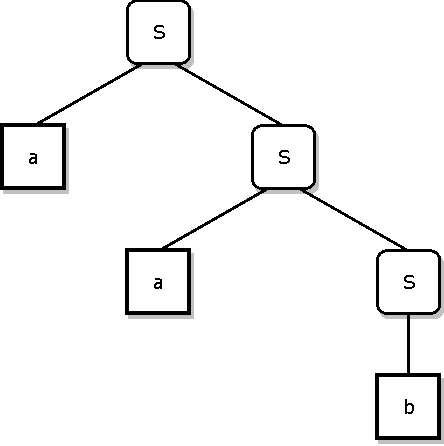
\includegraphics[width=5cm]{img/DerivacniStromDemo}
				\caption{Ukázka derivačního stromu}
			\end{figure}
		
			\paragraph{Nejednoznačné slovo}
			je takové slovo, pro které existuje v gramatice několik různých derivačních stromů. Pro příklad uveďme gramatiku obsahující sčítání a odčítání
			\Grammar{a,+,-}{S}{S}{S\rightarrow S+S,\allowbreak S\rightarrow S-S,\allowbreak S\rightarrow a} kde díky nejednoznačnosti není pevně dána přednost operací u slova $w=a+a-a$ (viz obrázek \ref{pic:ambiguousTree}).
			\begin{figure}[h!]
				\centering
				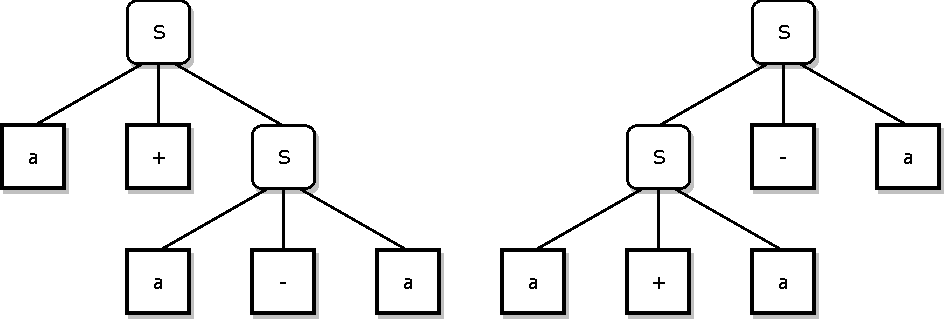
\includegraphics[width=10cm]{img/NejednoznacnyDerivacniStrom}
				\caption{Derivační stromy pro nejednoznačné slovo}
				\label{pic:ambiguousTree}
			\end{figure}
			\paragraph{Jednoznačná gramatika}
			je taková gramatika, která nemá v~generujícím jazyce ani jedno nejednoznačné slovo.
			
		
		\subsection{Deterministické bezkontextové gramatiky}
			Deterministické gramatiky, nebo také \LRk gramatiky, jsou gramatiky ekvivalentní s~modelem deterministického zásobníkového automatu. Jedná se o~podmnožinu jednoznačných gramatik \cite{Meduna:2014:FLC:2636678}. Jak již bylo řečeno, zásobníkový automat je model, který byl přiřazen právě k~bezkontextovým gramatikám jako jejich ekvivalent -- dokážou popsat stejnou množinu jazyků. Následující popis vychází z~materiálu \cite{Meduna:2014:FLC:2636678}.
			
			\paragraph{Deterministický stavový automat}
			je pětice $M=\left(Q, T, \delta, q_0, F\right)$. $Q$ je množina vnitřních stavů, $T$ je vstupní abeceda (ekvivalent terminálů), $\delta$ je zobrazení $Q\times X\rightarrow Q$, $q_0$ je počáteční stav automatu ($q_0\in Q$) a $F$ je množina koncových stavů. Automat na základě aktuálního stavu a dalšího znaku na vstupu přechází do stavu jiného, a to podle zobrazení $\delta$. Tento proces končí až ve chvíli, kdy je přečteno celé slovo. Pokud není pro vstupní symbol definována přechodová funkce, proces končí a říkáme, že automat slovo nepřijal. Pokud je po přečtení celého slova automat v~jednom z~koncových stavů (množina $F$), potom tvrdíme, že automat slovo přijal.
			\paragraph{Nedeterministický stavový automat}
			je deterministický stavový automat, pouze s~rozdílnou definicí zobrazení $\delta$. Pro jeho nedeterministickou verzi je zobrazení $\delta$ definováno jako $Q\times T\rightarrow {2}^{Q}$, kde ${2}^{Q}$ je potenční množina. To znamená, že na základě stavu a následujícího znaku vstupního slova může automat přejít do více stavů současně. Pro další znak slova se provádí stejný postup pro každý jednotlivý stav, a to nezávisle na ostatních stavech. Netederministický stavový automat slovo přijímá, jestliže alespoň jedna z~větví skončila v~koncovém stavu.
			\paragraph{Nedeterministický zásobníkový automat}
			je automat definovaný sedmicí $K=\left(Q, T, Z, \delta, q_0, Z_0, F\right)$. Od stavového automatu se liší abecedou zásobníku $Z$, počátečním symbolem zásobníku $Z_0 \in Z$ a pravidly $\delta$ tvaru $Q \times (T \cup \left\{\varepsilon\right\}) \times \theta_S \rightarrow Q \times \theta_E$ kde $\theta_S, \theta_E \in  {Z}^{\ast}$. Přechod probíhá na základě aktuálního stavu, dalšího znaku vstupního slova ~ na základě libovolného explicitního počtu znaků na zásobníku $\theta_S$. Tyto znaky jsou ze zásobníku odebrány, automat se přesune do nového stavu a vloží na zásobník libovolný (i~nulový) počet znaků $\theta_E$.\par
			Stejně jako u nedeterministického stavového automatu, paralelní přechody jsou na sebe navzájem nezávislé, tj. operace se zásobníkem u jednoho přechodu neovlivní stav zásobníku u zbylých přechodů. Automat končí ve chvíli, kdy není definována přechodová funkce, nebo kdy je přečteno celé vstupní slovo. Automat má dvě možnosti, jak může slovo přijmout. Stejně jako u~nedeterministického stavového automatu, nedeterministický zásobníkový automat slovo příjímá, jestliže jedna z~větví skončí v~koncovém stavu. Automat taktéž slovo přijímá, pokud alespoň jedna větev odebrala ze zásobníku všechny symboly a~přečetla celé vstupní slovo. O~tom, kterým způsobem nedeterministický zásobníkový automat slovo přijímá, se musíme rozhodnout při definici automatu.
			\paragraph{Deterministický zásobníkový automat}
			je zásobníkový automat, pro kte\-rý existuje v~každém stavu maximálně jeden přechod, a to pro libovolný vstupní symbol i pro libovolné slovo na zásobníku.
			Nedeterminismus u zásobníkového automatu je způsoben situací, při níž existují přechody vycházející ze stejného stavu na stejný vstupní symbol (resp. symbol \Eps), a sekvence symbolů $\theta_{S1}$ jednoho přechodu je předponou sekvence $\theta_{S2}$ přechodu druhého. Pro příklad uveďme přechody $(Q_1 , a , Z_1) = (Q_2 , \varepsilon)$ a $(Q_1 , a , Z_1 Z_2 ) = (Q_2 , \varepsilon)$. Je-li automat ve stavu $Q_1$, na vstupu je symbol $a$ a na zásobníku jsou symboly $Z_1 Z_2$, potom vyhovují oba přechody a zásobník se stává nedeterministickým.
			Stejně jako u~jeho nedeterministické verze, deterministický zásobníkový automat slovo přijímá, jestliže přečte celé slovo a~skončí v~koncovém stavu, nebo přečte-li celé slovo a~ze zásobníku odebere všechny symboly. Způsob přijetí je nutný definovat předem.
			\paragraph{Deterministické bezkontextové gramatiky}
			jsou gramatiky, pro které lze sestrojit deterministický zásobníkový automat.
			
			\vspace{1em}
			
			Determinismus u zásobníkového automatu je pro \LRk gramatiky (resp. \LRk parsery) klíčový. Dovoluje totiž parsování v~lineárním čase v~závislosti na délce slova. \LRk parsery byly prvně popsány Donald Knuthem,
			ale bylo od nich opuštěno z~důvodu velkých paměťových nároků na parsovací algoritmus. S~ohledem na zvyšující se výkon počítačů se k~tomuto algoritmu opět vracíme \cite{Chapman:1987:LPT:40693}.
			
			Pro libovolnou deterministickou bezkontextovou gramatiku lze sestrojit \LRk parser, jedná se tedy o nejuniverzálnější parser s~lineární časovou složitostí. Pro parsování je použita tzv. bottom-up metoda založená právě na fungování deterministického zásobníkového automatu \cite{Chapman:1987:LPT:40693}. 
			
			Zjednodušeně se na zásobník postupně vkládají znaky vstupního slova. Ve chvíli, kdy existuje pravidlo, které se derivuje na symboly v~zásobníku, je pravidlo použito a~symboly v~zásobníku jsou nahrazeny levou stranou pravidla. Tento postup nutně nemusí vést na deterministický zásobníkový automat. Aby kompiler věděl, které pravidlo použít, používá tzv. \MathSymb{LR parsing table}. Ta je předpočítaná a obsahuje vyhovující pravidla v závislosti na dalších znacích vstupního slova. Parser na základě \MathSymb{k} nepřečtených znaků vstupního slova a~aktuálního stavu zásobníku vyhledá v tabulce příslušné pravidlo, které použije (odtud \LRk parsery). Tím je zajištěn determinismus a lineární časová složitost \cite{Meduna:2014:FLC:2636678}. 
		
		\subsection{LL gramatiky}
			\label{sec:LLgrammars}
			\LLk gramatiky \cite{Blythe:1994:LLV:191033.191121} jsou podobně jako \LRk gramatiky založeny na fungování deterministického zásobníkového automatu, ale tentokrát tzv. top-down metodou. Ta nejprve vloží na zásobník startovací symbol. Existuje-li pravidlo, které přepisuje symbol na vrcholu zásobníku, je použito a symbol na zásobníku je nahrazen pravou stranou pravidla. Ve chvíli, kdy je symbol na vstupu stejný jako symbol na vrcholu zásobníku, je symbol ze zásobníku odebrán a~symbol ze vstupu přečten.
			
			Tento postup téměř jistě nevede na deterministický zásobníkový automat, protože je symbol expandován bez znalosti vstupu (tedy nedeterministicky). Proto \LLk parsery (podobně jako \LRk parsery) tvoří tzv. \MathSymb{LL parsing table}, která plní stejnou funkci (odtud \LLk parsery).
			
			\LLk gramatiky nejsou tak univerzální jako \LRk gramatiky (jsou jejich podmnožinou), protože se při parsování musí rozhodnout o~použití pravidla ještě před tím, než je jakýkoliv vstup přečten (na rozdíl od \LRk parserů, které se rozhodují až po přečtení). Na druhou stranu se díky tomu v \MathSymb{LL parsing table} zajímáme pouze o levou stranu pravidel, zatímco v \MathSymb{LR parsing table} je to strana pravá. To vede k menšímu počtu záznamů a~tím k~menší zátěži na paměť \cite{Blythe:1994:LLV:191033.191121}.
		
		\subsection{LR(0), \gls{gloss:SLR} a \gls{gloss:LALR} gramatiky}
			\MathSymb{LR(0)}, \MathSymb{SLR} a \MathSymb{LALR} gramatiky jsou zjednodušení \LRk gramatik \cite{Chapman:1987:LPT:40693}. Ačkoliv dokáže \LRk gramatika zpracovat libovolnou deterministickou gramatiku, paměťová složitost \LRk parserů byla v~minulosti příliš velká. \MathSymb{LR(0)} parsery fungují bez paměťové režie (parsery mají nulový náhled, tedy \MathSymb{LR parse table} není použita), ale mají malou vyjadřovací schopnost.
			
			Z~toho důvodu popsal Frank DeRemer dvě zjednodušené verze \LRk parserů, konkrétně Simple LR Parser (\MathSymb{SLR}) a~Look-Ahead LR Parser (\MathSymb{LALR}) \cite{Deremer:1969:PTL:888578}.
			Tyto parsery si ponechaly lineární časovou složitost, ale na rozdíl od \LRk parserů jsou méně náročné na paměť.
			
		\vfill
			
		Vzhledem k počtu skupin, které byly výše zmíněny, je přiložen graf (obrázek \ref{pic:contextfreeLanguages}) ukazující bezkontextové gramatiky, jejich rozdělení a vzájemnou inkluzi a~exkluzi jednotlivých podmnožin.
		
		\begin{figure}[h]
			\centering
			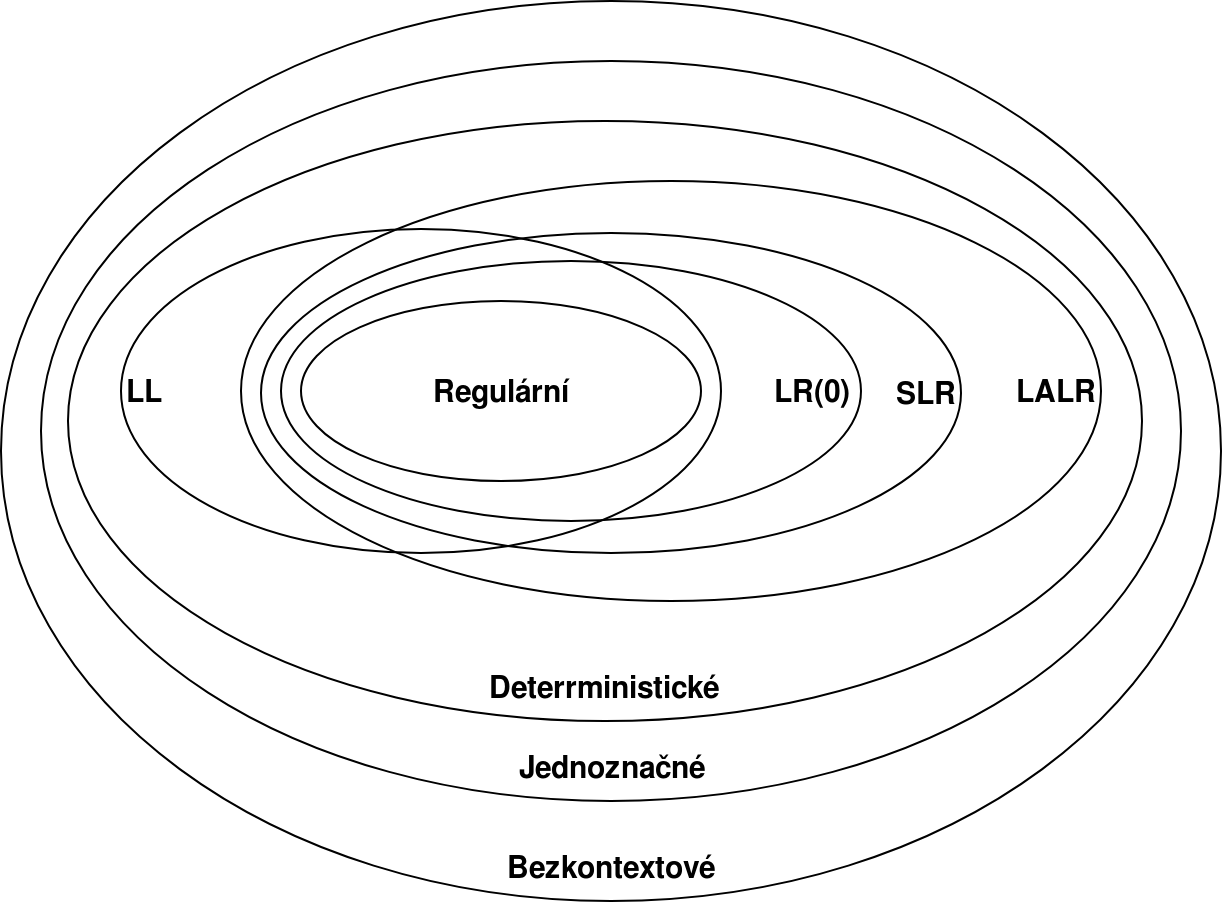
\includegraphics[width=8cm]{img/ContextFreeLanguageGroups}
			\caption{Rozdělení bezkontextových jazyků}
			\label{pic:contextfreeLanguages}
		\end{figure}
		
		S~již zmíněnými parsovacími metody se nebudeme dále zabývat, protože nejsou předmětem této práce. Byly vyjmenovány z důvodu, že na ně knihovna musí pamatovat pro budoucí rozšíření. Práce se dále zabývá \gls{gloss:CYK} algoritmem, který je detailněji popsán v~daůší části. Pro použití \gls{gloss:CYK} algoritmu je nutné mít gramatiku v~\gls{gloss:CNF} a~tomu se věnuje sekce \ref{sec:ChomskyNormalForm}.
		
	\section{Formální překlady}
		Překlad \cite{Aho:1969:TCF:800169.805425} je operace, která každému vstupu přiřazuje nějaký výstup. Překlady mezi různými světovými jazyky pravděpodobně není nutné zmiňovat, ale může se jednat i~o~převod matematických zápisů mezi prefixovou, postfixovou a~infixovou notací. Dalším příkladem je převod mezi číselnými soustavami nebo kódování (například binární data na Base64).
		
		\paragraph{Fomální překlad}
		je relace $Z\subseteq L\times V$, kde $L$ je libovolný jazyk a $V$ jazyk překladů. Relace přiřazuje každému slovu jazyka \MathSymb{L} jeho překlad patřící do \MathSymb{V}.
		\paragraph{Překladová gramatika}
		je \TranslateGrammarDef, \MathSymb{T} je množina terminálů (resp. vstupních symbolů), \MathSymb{N} je množina neterminálů, \MathSymb{D} je výstupní abeceda (disjunktní s~abecedou terminálů a~neterminálů), \MathSymb{S} je počáteční symbol a \MathSymb{R} je množina pravidel $R\subseteq{\left(T \cup N \cup D\right)}^{\ast}$.
		
		\vspace{1em}
		
		Do definice gramatik přibyla v~překladové gramatice výstupní abeceda (či množina výstupních symbolů). Výstupní symboly budeme dále v~textu označovat malými písmeny v~kruhu -- \circled{a}, \circled{x}.
		
		\paragraph{Homomorfismus}
		je zobrazení $h\subseteq X \times Y^\ast$, kde \MathSymb{X} a \MathSymb{Y} jsou abecedy.
		\paragraph{Rozšířený homomorfismus}
		je homomorfismus $h:X^*\times Y^*$ definovaný indukcí.
		$$h(\varepsilon)=\varepsilon$$
		$$h(xa)=h(x)h(a), x\in X^*, a\in X$$		
		\paragraph{Vstupní homomorfismus}
		je rozšířený homomorfismus, který nahrazuje všechny symboly $x\in D$ symbolem \Eps.
		\paragraph{Výstupní homomorfismus}
		je rozšířený homomorfismus, který nahrazuje všechny symboly $x\in T \cup N$ symbolem \Eps.
		
		\vspace{1em}
		
		Překlad zpravidla probíhá tak, že je naparsováno vstupní slovo (odtud vstupní homomorfismus) a podle použitých pravidel je výsledkem výstupní slovo (odtud výstupní homomorfismus). Samotný derivační strom (resp. větná forma) obsahuje jak vstupní, tak výstupní symboly.
		
		Předpokládejme \TranslateGrammarNoRuleSet{a,+,*}{S,A,P,K}{\circled{a},\circled{+},\circled{-}}{S}{R}, kde R:
		\begin{center}
			\begin{minipage}{.45\textwidth}
				\begin{lstlisting}[escapeinside={(*}{*)}]  
S (*$\rightarrow$*) a(*\circled{a}*)A
S (*$\rightarrow$*) a(*\circled{a}*)
K (*$\rightarrow$*) a(*\circled{a}*)(*\circled{$\ast$}*)A
K (*$\rightarrow$*) a(*\circled{a}*)(*\circled{$\ast$}*)
				\end{lstlisting}
			\end{minipage}
			\hfill
			\begin{minipage}{.45\textwidth}
				\begin{lstlisting}[escapeinside={(*}{*)}]  
A (*$\rightarrow$*) (*$\ast$*)Kz
A (*$\rightarrow$*) +P
P (*$\rightarrow$*) a(*\circled{a}*)(*\circled{+}*)A
P (*$\rightarrow$*) a(*\circled{a}*)(*\circled{+}*)
				\end{lstlisting}
			\end{minipage}
		\end{center}
	
		Pro vstupní slovo $w_i=a + a \ast a$ bude překlad $w_o=\circled{a}\circled{a}\circled{+}\circled{a}\circled{$\ast$}$. Derivační strom je v~příloze na obrázku \ref{fig:translateGrammar}.
		
		Ačkoliv by se to z~názvu \enquote{Překladové gramatiky} dalo usuzovat, tyto gramatiky ve skutečnosti nepřekládají programy do spustitelné podoby. Překladové gramatiky nejsou schopny dodat sémantickou stránku překladu, tedy to, jak se bude program chovat. K tomu slouží gramatiky atributované.
		
	\section{Atributované gramatiky}
		Již zmiňované parsovací metody řeší pouze skladbu vstupního slova -- jeho syntax. Jeho skladba má ovšem i~specifický význam -- hovoříme o~sémantickém významu. Následující kapitola vychází primárně z~materiálu \cite{4308414}.
		
		\paragraph{Syntax}
		je množina pravidel a principů, které řídí strukturu věty daného jazyka, zpravidla definicí povolených kombinací symbolů. Syntax zajišťuje ověření, zda je vstupní věta správně strukturována.
		
		\vspace{1em}
		
		Správnou syntaxi vstupní věty vynutíme právě použitím gramatik. Ve většině případů nechceme pouze ověřit, zda je vstupní věta syntakticky správně, ale požadujeme její další zpracování. Pokud již máme vytvořenou syntaxi, nezpracováváme samotný text, ale jeho význam. Z~tohoto důvodu se snažíme text během procesu parsování převést do jiných struktur, vhodnějších pro další zpracování. Jednou z~takových struktur je abstraktní syntaktický strom.
		
		\paragraph{Abstraktní syntaktický strom}
		je stromovou reprezentací abstraktní syntaktické struktury zdrojového kódu. Uzly abstraktního derivačního stromu reprezentují konstrukce ve zdrojovém kódu. Abstraktní syntaktický strom dodržuje pravidla syntaxe, uzly a hrany derivačního stromu jsou převedeny do struktur vhodných k~dalšímu zpracování. Samotná podoba těchto struktur se může v~závislosti na dalším zpracování lišit. Svým způsobem se jedná o~reprezentaci derivačního stromu datovými strukturami. Abstraktní syntaktický strom budeme dále v textu označovat jako \gls{gloss:AST} (z~anglického Abstract Syntax Tree).
		
		\vspace{1em}
			
		Abstraktní syntaktický strom reprezentuje syntaktickou stránku programovacích jazyků. Respektuje správnou syntax, ale nedefinuje význam, tedy sémantiku. Sémantika musí být přidána dodatečně.
		
		\paragraph{Sémantika}
		přidává význam syntakticky korektním větám. V kontextu programovacích jazyků sémantika popisuje postup, který zařízení provádí během spuštění daného programu.
		
		\vspace{1em}
		
		Pro definici atributované gramatiky, která dodává sémantický význam, potřebujeme nadefinovat další pojmy.
		
		\paragraph{Atribut}
		je veličina, která může nabývat hodnot z~definované množiny. Atribut můžeme přirovnat k~proměnné v~programovacích jazycích.
		\paragraph{Atributovaný symbol}
		je symbol abecedy, ke kterému je přiřazena konečná množina atributů. Tato množina může být i prázdná. Přístup k~atributu $a$ přiřazeného symbolu $x$ budeme značit jako $x.a$. Atribut $a$ s hodnotou \MathSymb{1} pro symbol $x$ budeme značit jako $x.a[1]$. Jestliže bude atributů více, budeme je oddělovat tečkou, tedy symbol $x$ s jeho atributy $a=1$ a $b=2$ budeme značit jako $x.a[1].b[2]$.
		\paragraph{Atributovaný řetězec}
		nad abecedou $A$ je řetězec atributovaných symbolů z~$A$.
		\paragraph{Atributovaný překlad}
		je relace ${T}^{\ast} \times {D}^{\ast}$, kde ${T}^{\ast}$ je množina vstupních atributovaných řetězců a ${D}^{\ast}$ množina výstupních atributovaných řetězců.
		
		\vspace{1em}
		
		Vztáhneme-li kontext zpět na gramatiky a~\gls{gloss:AST}, můžeme každému terminálu a~neterminálu přiřadit množinu atributů. Dále budeme uvažovat pouze o jednom atributu \MathSymb{v}. Pomocí atributů můžeme mít několik způsobů, jak reprezentovat číslo 253.
		\begin{itemize}
			\item Neterminál $x$ reprezentující celé číslo jako $x.v[253]$.
			\item Neterminál $x$ reprezentující cifru a pravidla $c \rightarrow x c, c\rightarrow\varepsilon$, kde $c$ reprezentuje celé číslo. Pro číslo 253 by 
			$c\Rightarrow x_1c \Rightarrow x_1x_2c\Rightarrow x_1x_2x_3c\Rightarrow x_1x_2x_3$, kde $x_1.v[2], x_2.v[5], x_3.v[3]$.
			\item Neterminály $x_0,x_1,\cdots,x_9$ s pevně danými atributy $x_k.v[k]$.
		\end{itemize}
	
		Konkrétní výběr se může lišit podle způsobu dalšího zpracování a kontextu gramatiky. Z~pohledu sémantiky bychom ovšem potřebovali, abychom ke všem třem variantám přistupovali stejně, tedy očekáváme, že kořen \gls{gloss:AST} reprezentující číslo bude mít atribut obsahující hodnotu čísla. Přitom chceme zůstat nezávislí na způsobu reprezentace.
		
		Jak je z~popisu patrné, hodnoty neterminálních atributů nemůžeme volit pevně, ale musí se měnit v závislosti na pozici v~\gls{gloss:AST} -- nejčastěji na základě atributů potomků nebo rodiče. Toho dosáhneme sémantickými pravidly.
		
		\paragraph{Sémantická funkce}
		je funkce, která přiřadí atributu hodnotu na základě jiných atributů. Jedná se o funkci $f=(a_1,a_2,\cdots,c_n)$, kde $a_1,a_2,\cdots,c_n$ jsou atributy, na kterých je funkce závislá. Funkce je zapsána libovolným, pro danou situaci vhodným způsobem (například programovacím jazykem uvnitř překladače).
		\paragraph{Sémantické pravidlo}
		je pravidlo, které má navíc sémantickou funkci.
		\paragraph{Atributovaná překladová gramatika}
		je \AttributTranslateGrammarDef, kde \MathSymb{N} je abeceda neterminálů, \MathSymb{T} je abeceda terminálů, \MathSymb{D} je abeceda výstupních symbolů, \MathSymb{SR} jsou sémantické pravidla, \MathSymb{S} je počáteční symbol $S\in N$, \MathSymb{A} je množina atributů a \MathSymb{V} je zobrazení $V\subseteq\left(T\cup N\right)\times{A}^\ast$, tedy množina přiřazující každému terminálu či neterminálu množinu atributů.
		\paragraph{Dědičný atribut}
		je atribut \MathSymb{v} symbolu \MathSymb{x}, jehož sémantická funkce \MathSymb{f} závisí pouze na dědičných atributech symbolu \MathSymb{x} nebo na dědičných atributech jeho rodiče.
		\paragraph{Syntetizovaný atribut}
		je atribut \MathSymb{v} symbolu \MathSymb{x}, jehož sémantická funkce závisí pouze na syntetizovaných či dědičných atributech symbolu \MathSymb{x}, nebo na syntetizovaných či dědičných atributech jeho potomků.
		\paragraph{Vyhodnocení atributů}
		je proces, během kterého jsou vyhodnoceny sémantické funkce a nastaveny hodnoty atributů. Pro správné vyhodnocení musí být splněno:
		\begin{itemize}
			\item hodnoty dědičných atributů počátečního symbolu musí být známy,
			\item hodnoty syntetizovaných atributů vstupních symbolů musí být známy,
			\item hodnota atributu musí záviset pouze na již známých hodnotách atributů.
		\end{itemize}
		
		\vspace{1em}
		
		Poslední bod vylučuje situace, které by mohly vést k~zacyklení výpočtu. Nejjednodušším příkladem je atribut \MathSymb{a} závisející na atributu \MathSymb{b}, přitom atribut \MathSymb{b} zpětně závisí na atributu \MathSymb{a}. Pokud budou atributy záviset pouze na již známých hodnotách atributů, k~zacyklení dojít nemůže.
		
		Jako příklad atributované gramatiky uvedeme gramatiku vyhodnocující aritmetické operace \MathSymb{+} a \MathSymb{$\ast$}. Pro všechny symboly předpokládáme syntetizovaný atribut \MathSymb{v}. Pravidla lze nalézt v~tabulce \ref{tab:attributed_arithmetic}. Symboly, které se v~pravidlu vykytují opakovaně je nutné v~sémantických funkcích rozlišit, proto jsou symboly indexovány. V~obrazové příloze je na obrázku \ref{fig:attributedGrammar} zobrazeno vyhodnocení vstupního slova $a.v[3]+a.v[2]*a.v[4]$.
		
		\begin{table}[h!]
			\centering
			\caption{Atributovaná gramatika vyhodnocující aritmetické operace}	
			\label{tab:attributed_arithmetic}
			\begin{tabular}{| l | l |}
				\hline
				\textbf{Pravidlo} & \textbf{Sémantika} \\
				\hline
				\MRule{S}{E} & $S.v = E.v$ \\
				\hline
				\MRule{E_1}{E_2 + T} & $E_1.v = E_2.v + T.v$ \\
				\hline
				\MRule{E}{T} & $E.v = T.v$ \\
				\hline
				\MRule{T_1}{T_2 * F} & $T_1.v = T_2.v * F.v$ \\
				\hline
				\MRule{T}{F} & $T.v = F.v$ \\
				\hline
				\MRule{F}{a} & $F.v = a.v$ \\
				\hline
				\MRule{F}{\left(E\right)} & $F.v = E.v$ \\
				\hline
			\end{tabular}		
		\end{table}
		
	\section{Chomského normální forma}
		\label{sec:ChomskyNormalForm}
		Chomského normální forma (\gls{gloss:CNF}) je speciální formát gramatiky vyžadována \gls{gloss:CYK} algoritmem. Libovolnou bezkontextovou gramatiku lze převést do \gls{gloss:CNF} \cite{Meduna:2014:FLC:2636678}.
		Pro tuto transformaci jsou známy a popsány algoritmy, které jsou blíže rozebrány v~další kapitole.
		
		Chomského normální forma povoluje pouze pravidla následujících typů:
		\begin{itemize}
			\item $A \rightarrow B C$,
			\item $A \rightarrow a$,
			\item $S \rightarrow \varepsilon$, kde \Nonterm{S} se nesmí vyskytovat na pravé straně žádného pravidla.
		\end{itemize}
	
		Před tím, než blíže popíšeme algoritmy pro transformaci gramatik, sloužící k~převodu do \gls{gloss:CNF}, potřebujeme dodefinovat další pojmy, které se v~kontextu těchto transformací vyskytují. Pojmy vycházejí z~materiálu \cite{Meduna:2014:FLC:2636678}.
		
		\paragraph{Negenerující symbol}
		je symbol, který negeneruje žádnou větu. Pokud je počáteční symbol \MathSymb{S} negenerující, gramatika negeneruje žádné slovo, a~tedy generuje prázdný jazyk.
		\paragraph{Dostupný symbol}
		je symbol, který se vyskytuje v~nějaké větné formě. Formálně se jedná o symbol $X: S \Rightarrow\alpha X \beta; \alpha,\beta\in\TermNontermIter$.
		\paragraph{Nedostupný symbol}
		je symbol, který není dostupný.
		\paragraph{\EpsS pravidlo}
		je pravidlo ve tvaru $X\rightarrow\varepsilon$.
		\paragraph{Zkracující pravidlo}
		je pravidlo, jehož počet symbolů na levé straně je větší než počet symbolů na straně pravé. Délka \EpsS symbolu je považována za nulovou.
		\paragraph{Zkracující gramatika}
		je gramatika, která má alespoň jedno pravidlo zkracující.
		\paragraph{Symbol derivovatelný na \EpsS přímo}
		je takový symbol \MathSymb{X}, pro nějž platí $X{\Rightarrow}^{1}\varepsilon$. V~gramatice musí existovat pravidlo $X\rightarrow\varepsilon$.
		\paragraph{Symbol derivovatelný na \EpsS nepřímo}
		je takový symbol \MathSymb{X}, pro nějž platí $X{\Rightarrow}^{i}\varepsilon;i>1$.
		\paragraph{Jednoduché pravidlo}
		je pravidlo tvaru $A \rightarrow B$, tedy pravidlo přepisující neterminál na neterminál.
		
		
		
	

\chapter{Operace s gramatikami}
	
	Operace s~gramatikami můžeme obecně rozdělit na transformační (mění podobu gramatiky) a~parsovací (zpracovávají text). V~rámci parsovacích operací se snažíme o~nejefektivnější validaci vstupu za současného převodu do struktur vhodných pro další zpracování. Tyto struktury se mohou v závislosti na úrovni abstrakce a potřebě zasahovat do procesu zpracování měnit. Běžně používanou reprezentací je již zmiňovaný abstraktní syntaktický strom, kterým se budeme zabývat dále v práci. Další běžně známou reprezentací je Java bytecode, který je překládán až na cílové platformně při spuštění aplikace. \gls{gloss:GCC} například podporuje několik reprezentací: Register Transfer Language, \gls{gloss:LLVM}, Static single assignment form a další.
	
	Z~hlediska transformačních operací jde o~vytvoření nové, optimalizované gramatiky, která bude generovat stejný jazyk jako gramatika původní. To je případ i algoritmů pro převod gramatiky do \gls{gloss:CNF}. Tyto transformace jsou známé a~popsané. Transformace, které mění generující jazyk, jsou méně obvyklé, protože vyžadují širší kontext a náročnou intelektuální práci, kterou je téměř nemožno algoritmizovat. Tyto transformace dovolují změnit gramatiku do podoby, kterou je možno parsovat rychlejším parsovacím algoritmem. Pokud je generovaný jazyk podmnožinou (resp. nadmnožinou nebo kombinací) původního jazyka, musí se rozdíly zpracovat v~pozdějších fázích překladu.
	
	\section{Problémy transformací}
	
	Na druhou stranu i transformace, neměnící generovaný jazyk, mohou měnit syntaktickou strukturu. To je nežádoucí, protože v~rámci atributovaných gramatik (či jiného způsobů zpracování) předpokládáme strukturu definovanou naší gramatikou. Aplikováním transformací se gramatika (a tím i~syntaktická struktura) změní.
	
	\begin{figure}
	\begin{lstlisting}[escapeinside={(*}{*)}]
STATEMENT (* $\rightarrow$ *) if CONDITION STATEMENT STATEMENT
STATEMENT (* $\rightarrow$ *) (* \dots *)
CONDITION (* $\rightarrow$ *) (* \dots *)
	\end{lstlisting}
	\caption{Ukázka gramatiky představující \enquote{if statement}}
	\label{pic:ifStatementDemo}
	\end{figure}

	\begin{figure}
		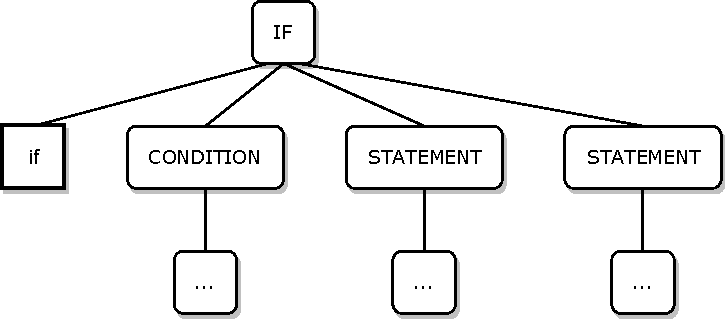
\includegraphics[width=0.45\textwidth]{img/DemoIfStatement}
		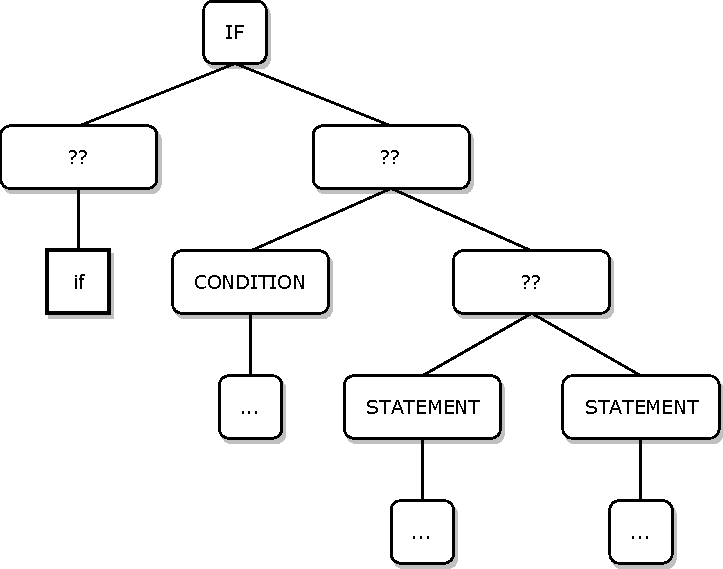
\includegraphics[width=0.45\textwidth]{img/DemoIfStatementWithTransformation}
		\captionof{figure}{Očekávaný a~reálný syntaktický strom pro \enquote{if statement}}
		\label{pic:ifStatemenAST}
	\end{figure}
	
	Pro představu budeme situaci demonstrovat na jednoduché gramatice (obrázek \ref{pic:ifStatementDemo}), převedené do \gls{gloss:CNF}.
	Po naparsování vstupu bychom očekávali výstup jako na obrázku \ref{pic:ifStatemenAST} vlevo. Ale vzhledem k~transformacím gramatiky bude výsledek odlišný (obrázek \ref{pic:ifStatemenAST} vpravo).
	
	To je z~hlediska sémantické analýzy komplikace, protože v~době tvorby gramatiky netušíme, jak bude gramatika transformovaná a to nám brání v~dodání sémantického významu pro modifikovaný \gls{gloss:AST}. Z~tohoto důvodu musí knihovna obsahovat i funkcionalitu ke zpětné rekonstrukci syntaktického stro\-mu podle původní netransformované gramatiky.
	
	\section{Převod do Chomského normální formy} 
	
	Práce dále popisuje všechny transformace i s~jejich pseudokódem. Po pseudokódu následuje popis zpětné transformace (pokud dává smysl), možné dopady na původní transformaci a popis změn v parsovacím procesu. Jednotlivé algoritmy, jejich popis a~pseudokód vychází z~materiálu \cite{Meduna:2014:FLC:2636678}.
	
	\subsection{Odstranění negenerujících symbolů}
	
	Vhodným příkladem může být gramatika pouze s~jediným pravidlem $S \rightarrow x S$. Všechny větné formy generované takovou gramatikou obsahují neterminál, generovaný jazyk je tedy prázdný.
	
	Odstranění negenerujících symbolů nemění syntaxi gramatiky (protože odstraněná část se nemůže vyskytnout v~žádné větné formě generujícího slova), ale zjednodušuje ji a tím snižuje časové a paměťové nároky na algoritmy, které dále s~gramatikou pracují.
	
	Algoritmus pro odstranění negenerujících symbolů si drží množinu symbolů, které tvoří libovolnou větu. Na počátku jsou v~této množině pouze terminály. Algoritmus poté hledá pravidla, které se přepíší na již generující symboly. Pokud takové pravidlo nalezne, přidá symbol na levé straně pravidla mezi generující symboly a postup opakuje.
	
	Algoritmus končí ve chvíli, kdy jsou zpracována všechna pravidla a žádný další generující symbol není přidán. Algoritmus poté z~gramatiky vymaže všechny negenerující symboly a s~nimi i všechna pravidla, která tyto symboly obsahují. Za předpokladu, že je gramatika konečná, algoritmus skončí po konečném počtu kroků. Pseudokód algoritmu je kód \ref{alg:removeNongeneratingSymbols}.
	
	\begin{listing}[h]
		\begin{minted}[tabsize=3]{text}
odstranění_negenerujících_symbolů(gramatika):
	generující = gramatika.terminály
	opakuj dokud se generující množina nezměnila:
		pro každé pravidlo v gramatice:
			jsou-li všechny symboly pravé strany generující:
				generující.přidej(pravá strana pravidla)

	odstranit = gramatika.nonterminály - generující
	gramatika.odstran(odstranit)
		\end{minted}
		\caption{Pseudokód algoritmu odstraňující negenerující symboly}
		\label{alg:removeNongeneratingSymbols}
	\end{listing}
	
	Pro algoritmus není nutné implementovat zpětnou transformaci, protože nemění syntaktickou strukturu gramatiky, ale pouze gramatiku optimalizuje.
	
	Speciální situace nastává ve chvíli, kdy algoritmus označí počáteční symbol gramatiky jako negenerující. V takovém případě gramatika generuje prázdný jazyk a v dalších algoritmech nemusíme pokračovat.
	
	\subsection{Odstranění nedostupných symbolů}
	Odstranění nedostupných symbolů je, stejně jako odstranění negerujících symbolů, pouze optimalizační technika, která snižuje velikost gramatiky a~tím i~časové a paměťové nároky  dalších algoritmů, které s~gramatikou pracují.
	
	Algoritmus pro odstranění nedostupných symbolů je velmi podobný algoritmu pro odstranění negenerujících symbolů, pouze prochází gramatiku v~opačném směru. Algoritmus si drží množinu dostupných symbolů, do které na počátku vloží počáteční symbol. Poté prochází pravidla a~pro ta, jejichž levá strana je obsažena v~množině, vloží do množiny dostupných symbolů také všechny symboly pravé strany. Pseudokód je kód \ref{alg:removeNonreachableSymbols}.
	
	\begin{listing}[h]
		\begin{minted}[tabsize=3, breaklines]{text}
odstranění_nedostupných_symbolů(gramatika):
	dostupné = gramatika.počáteční_symbol
	opakuj dokud se množina dostupných symbolů nezměnila:
		pro každé pravidlo v gramatice:
			je-li levá strana pravidla v dostupné:
				dostupné.přidej(pravá strana)

	odstranit = gramatika.nonterminály
	            + gramatika.terminály 
	            - dostupné
	gramatika.odstran(odstranit)
		\end{minted}
		\caption{Pseudokód algoritmu odstraňující nedostupné symboly}
		\label{alg:removeNonreachableSymbols}
	\end{listing}
	
	Na rozdíl od algoritmu pro odstranění negenerujících symbolů mohou být během běhu algoritmu odstraněny i terminály. Terminály mohou být odstraněny všechny, a to ve chvíli, kdy gramatika generuje pouze \Eps.
	
	\subsection{Odstranění \EpsS pravidel}
	
	Bezkontextové gramatiky mají obecný tvar pravidla $X\rightarrow\TermNontermIter$. V~takové gramatice lze (na rozdíl od gramatik regulárních a kontextových) derivovat libovolný symbol na \EpsS (obsahuje-li gramatika příslušná pravidla). To by komplikovalo parsovací proces, protože by byla gramatika zkracující.
	
	Cílem algoritmu je transformovat gramatiku s~\Eps~pravidly na gramatiku bez \Eps~pravidel a~tím ji udělat nezkracující.
	
	Algoritmus nejprve nalezne všechny neterminály, které jsou přímo nebo nepřímo derivovatelné na \Eps. Postup je velmi podobný jako u algoritmu pro odstranění negenerujících symbolů, pouze s~tím rozdílem, že na počátku algoritmu vložíme do generujících symbolů pouze \Eps. Pseudokód je kód \ref{alg:searchEpsilonGenerating}.
	
	\begin{listing}[h]
		\begin{minted}[tabsize=3]{text}
nalezení_neterminálů_přepisovatelných_na_epsilon(gramatika):
	generujici = vytvoř množinu
	opakuj dokud se generujici množina nezměnila:
		pro každé pravidlo v gramatice:
			jsou-li všechny symboly pravé strany přepisovatelné:
				generujici.přidej(pravá strana)

	vrať přepisovatelné
		\end{minted}
		\caption{Pseudokód algoritmu hledající neterminály generující \Eps}
		\label{alg:searchEpsilonGenerating}
	\end{listing}
	
	Poté algoritmus projde všechna pravidla. Pravidla, která se přímo přepisují na \Eps~jsou z~gramatiky vyloučena. Touto operací dojde k modifikaci gramatiky a tím i ke změně generujícího jazyka. To je pro další práci nepřípustné, protože jako výstup požadujeme gramatiku generující stejný jazyk.
	
	\paragraph{Vyloučení pravidla}
	je proces, který z gramatiky odebere pravidlo bez toho, aniž by byl změněn generující jazyk. Nechť \GrammarDef\space je bezkontextová gramatika a v~ní pravidlo $\rho=A\rightarrow\alpha$, které vyloučíme. Jestliže ke všem pravidlům $X\rightarrow\gamma A \delta$ přidáme pravidlo $X\rightarrow\gamma\alpha\delta$, potom se generovaný jazyk nezmění.
	
	\vspace{1em}
	
	Věta nám říká, že nahradíme-li ve všech pravidlech neterminál, který je na levé straně vyloučeného pravidla, pravou stranou vyloučeného pravidla, poté gramatika popisuje stejný jazyk. Pseudokód je kód \ref{alg:removeRule}.
	
	\begin{listing}[h]
		\begin{minted}[tabsize=3]{text}
odstraň_pravidlo(gramatika, pravidlo):
	gramatika.odstraň(pravidlo)
	pro každé pravidlo p_1 v gramatice:
		pro každý symbol v p_1.pravá_strana:
			jestliže symbol = pravidlo.levá_strana:
				nové = nahraď symbol pravou stranou pravidla
				gramatika.přidej(nové)
		\end{minted}
		\caption{Pseudokód algoritmu odstraňující pravidlo}
		\label{alg:removeRule}
	\end{listing}
	
	V našem případě odstraňujeme pouze \EpsS pravidla (pravidla typu $X\rightarrow\varepsilon$). Během odstranění se modifikovaná pravidla zkracují (například z~pravidel $\left\{\right.A\rightarrow B,$ $B\rightarrow\varepsilon\left.\right\}$ vznikne $\left\{A\rightarrow B, A\rightarrow\varepsilon\right\}$), může se tedy stát, že vznikne nové \EpsS pravidlo. Algoritmus proto opakuje postup tak dlouho, dokud v~gramatice existují \EpsS pravidla. Pseudokód je kód \ref{alg:removeEpsilonRules}.
	
	\begin{listing}[h]
		\begin{minted}[tabsize=3]{text}
odstranění_epsilon_pravidel(gramatika):
	dokud v gramatice existují epsilon pravidla:
		pravidlo = najdi_epsilon_pravidlo(gramatika)
		odstraň_pravidlo(pravidlo)
		\end{minted}
		\caption{Pseudokód algoritmu odstraňující \EpsS pravidla}
		\label{alg:removeEpsilonRules}
	\end{listing}
	
	Tato verze algoritmu má velkou časovou složitost, protože opakovaně prochází všechna pravidla v~gramatice. Algoritmus lze optimalizovat použitím fronty a množiny symbolů derivovatelných na \Eps. Algoritmus poté prochází každé pravidlo pouze jednou.
	
	%			\begin{listing}[h]
	%				\begin{minted}[tabsize=3]{text}
	%odstranění_epsilon_pravidel(gramatika):
	%	přepisovatelné = nalezení_neterminálů_na_epsilon(gramatika)
	%	pravidla = vytvoř_frontu(gramatika.pravidla)
	%	dokud fronta pravidla není prázdná:
	%		pravidlo = další_prvek_ve_frontě(pravidla)
	%		pokud se praidlo.pravá_strana rovná epsilon:
	%			gramatika.odstraň(pravidlo)
	%			opakuj
	%		pro každý symbol v pravidlo.pravá_strana:
	%			pokud je symbol přepisovatelný:
	%				nové = vytvoř_pravidlo_bez_symbolu(pravidlo, symbol)
	%				gramatika.přidej(nové)
	%				pravidla.přidej(nové)
	%			\end{minted}
	%			\caption{Pseudokód optimalizovaného algoritmu odstraňující \EpsS pravidla}
	%		\end{listing}		
	
	Pro algoritmus odstranění \EpsS symbolů již potřebujeme algoritmus zpětné transformace syntaktického stromu. Při transformaci se pro nově vytvořená pravidla (tedy pravidla s odstraněným \EpsS symbolem) uloží pravidlo, ze kterého nové pravidlo vzniklo, a symbol, který byl přepsán na \Eps. Na základě těchto informací je algoritmus schopen určit originální pravidlo a syntaktický strom transformovat tak, aby odpovídal originální gramatice.
	
	\subsection{Odstranění jednoduchých pravidel}
	
	Algoritmus pro odstranění jednoduchých pravidel je podobný tomu pro odstranění \Eps~pravidel. Algoritmus ve své nejjednodušší implementaci vylučuje jednoduchá pravidla až do doby, pokud v~gramatice ještě nějaká existují. Optimalizovaná verze algoritmu má několik kroků, ale má nižší časové a~paměťové nároky. Jedná se o~pseudokód \ref{alg:removeUnitRules}.
	
	\begin{enumerate}
		\item
		Algoritmus vytvoří tranzitivní uzávěr jednoduchých pravidel.
		\item
		Algoritmus odstraní z~gramatiky všechna jednoduchá pravidla.
		\item
		Algoritmus prochází zbylá pravidla a~vybere ta, pro která v~gramatice existuje neterminál derivovatelný jednoduchými pravidly na levou stranu procházeného pravidla.\par
		Dále předpokládejme, že mluvíme o~obecném pravidlu $\Rule{X}{Ab}$ a~neterminálu $Z$ takovém, že existuje derivce $Z \Rightarrow X$ za použití pouze jednoduchých pravidel.
		\item
		Algoritmus vytvoří nové pravidlo. Na levé straně pravidla bude procházený neterminál a~na pravé straně pravá strana procházeného pravidla. Algoritmus tedy vytvoří pravidlo $\Rule{Z}{Ab}$.
		\item
		Vytvořené pravidlo přidá do gramatiky
	\end{enumerate}
	
	\begin{listing}
		\begin{minted}[tabsize=3]{text}
odstranění_jednoduchých_pravidel(gramatika):
	uzávěr = tranzitivní uzávěr jendoduchých pravidel
	pro každé pravidlo p_1 gramatiky:
		jestliže je p_1 jednoduché:
			gramatika.odstraň(p_1)
			pokračuj s dalším pravidlem
		pro každý neterminál n_1:
			pokud lze derivovat n_1 na p_1.levá_strana
				nové = pravidlo(n_1, p_1.pravá_strana)
				gramatika.přidej(nové)
		\end{minted}
		\caption{Pseudokód algoritmu odstraňující jednoduchá pravidla}
		\label{alg:removeUnitRules}
	\end{listing}
	
	Při algoritmu zpětné transformace je nutné pro nově vytvořené pravidlo uložit sérii jednoduchých pravidel, na základě kterých bylo pravidlo vytvořeno. Algoritmus dokáže podle této informace určit, která jednoduchá pravidla byla použita při odstranění, a z~toho vyvodit správnou podobu syntaktického stromu.
	
	\subsection{Převod na Chomského normální tvar}
	
	Připomeňme, že \gls{gloss:CNF} vyžaduje pravidla ve třech podobách:
	\begin{itemize}
		\item $A \rightarrow B C$,
		\item $A \rightarrow a$,
		\item $S \rightarrow \varepsilon$.
	\end{itemize}
	Po dokončení předchozích algoritmů máme jistotu, že se v gramatice nevykytuje pravidlo derivující se na \EpsS nebo jednoduchá pravidlo. Transformace do \gls{gloss:CNF} již probíhá jednoduše podle následujícího postupu.
	\begin{itemize}
		\item Pravidla vyhovující CNF ponecháme.
		\item Pravidla tvaru $A\rightarrow\alpha a \beta$ nahradíme pravidly $\left\{A\rightarrow\alpha a' \beta,\allowbreak a'\rightarrow a\right\}$ kde $a$~je terminál a~$a'$ je nový neterminál, dosud v~gramatice nepoužitý.
		\item Pravidla delší než dva neterminály rozdělíme vytvořením nových neterminálů a pravidel. Pravidlo $$A\rightarrow B_1 B_2 \cdots B_k$$ 
		rozdělíme na 
		\begin{flalign*}
				\left\{\right.
				&
				A\rightarrow B_1 \left<B_2\cdots B_k\right>, 
				\left<B_2\cdots B_k\right>\rightarrow B_2 \left< B_3\cdots B_k\right>, 
				\cdots, 
				&&\\
				&
				\left<B_{k-2}B_{k-1}B_k\right>\rightarrow B_{k-2} \left<B_{k-1}B_k\right>,
				\left<B_{k-1}B_k\right>\rightarrow B_{k-1} B_k
				\left.\right\} 
				&&
		\end{flalign*}
		kde $\left<\cdots\right>$ jsou nové neterminály, dosud v~gramatice nepoužité.
	\end{itemize}
	
	Pro algoritmus zpětné rekonstrukce nám postačí ukládat, o který ze dvou bodů výše se jedná, současně s pravidlem, ze kterého bylo nové pravidlo vytvořeno. Poté stačí uzel v syntaktickém stromu nahradit jeho správným ekvivalentem. V případě druhého bodu nahradíme uzel samotným terminálem, ve třetím případě (rozdělení pravidla) získáme zbytek neterminálů jako potomky pravého potomka.
	
	\section{Cocke-Younger-Kasami algoritmus}
	
	Cocke-Younger-Kasami algoritmus \cite{Younger1967} (nebo též \gls{gloss:CYK}) je jeden z parsovacích algoritmů pro bezkontextové gramatiky. Na rozdíl od zmíněných parsovacích algoritmů (jako LL a LR algoritmy) je schopen zpracovat libovolnou bezkontextovou gramatiku včetně nejednoznačné. Algoritmus je v takovém případě nedeterministický, ale konečný a~\gls{gloss:CYK} je schopen vstupní slovo naparsovat. Jedná se o~hlavní vlastnost, kvůli které byl algoritmus pro tuto práci vybrán.
	
	Jeho nevýhodou je zvýšená časová a paměťová náročnost. Časová složitost je v~nejhorším případě $\mathcal{O}(n^3 \cdot |G|)$, kde $|G|$ je počet pravidel v gramatice a $n$ je délka vstupního slova. Paměťová složitost je v nejhorším případě $\mathcal{O}(n^2 \cdot |G|)$. Další nevýhodou je neschopnost odhalovat chyby. Algoritmy pracující se slovem lineárně jsou schopny označit konkrétní symbol nevyhovující definici gramatiky. \gls{gloss:CYK} algoritmus odhalí nevalidní vstup, ale vzhledem k~jeho konstrukci není schopen určit místo, na kterém k~chybě došlo.
	
	\gls{gloss:CYK} algoritmus je založen na dynamickém programování. Algoritmus nej\-dří\-ve najde neterminály, které se přímo derivují na terminály vstupního slova (tj. použije všechny možné $X\rightarrow a$ pravidla). Algoritmus dále hledá všechny neterminály, které se derivují na podslova délky $2,3,\cdots,n$ obsažené ve vstupním slovu. Přitom využívá faktu, že slovo délky $k$ jsou dvě slova délek $(k-1,1),(k-2,2),\cdots,(2,k-2),(1,k-1)$. Pokud se v neterminálech, které generující celé vstupní slovo, vykytuje startovací symbol, potom je vstup úspěšně naparsován a algoritmus může vytvořit syntaktický strom.
	
	Běh algoritmu budeme dále v~textu demonstrovat tabulkou. První řádek tabulky budou neterminály generující vstupní slovo (tedy slovo délky $n$), druhý řádek část slova délky $n-1$, třetí řádek část slova délky $n-2$ atd. Na posledním řádku tabulky budou neterminály, které se přímo derivují na symboly vstupního slova.
	
	Proces budeme demonstrovat na gramatice \Grammar{a,b}{S,A,B,C}{S}{
		S \rightarrow A B,
		S \rightarrow B C,
		A \rightarrow B A,	
		A \rightarrow a,
		B \rightarrow C C,
		B \rightarrow b,
		C \rightarrow A B,
		C \rightarrow a,
	} \\ a slovu $w=aaba$.
	
	Algoritmus nejdříve zjistí, které neterminály se přímo derivují na symboly slova (například neterminály $A$ a $C$ se derivují na $a$). Ve druhém kroku tvoří slovo délky 2. Například neterminál $B\Rightarrow CC\Rightarrow aa$. Ve třetím kroku tvoří slova délky 3, tzn. kombinace slova délky 1 a slova délky 2 nebo slovo délky 2 a~slovo délky 1. Pro neterminál $B$ se použilo pravidlo $B\rightarrow CC$, kde první neterminál $C$ je~na třetím řádku a druhém sloupci (slovo délky 2) a druhý neterminál $C$ na čtvrtém a řádku čtverém sloupci (slovo délky 1). Neterminál $B$ skutečně generuje slovo délky 3, tedy $B\Rightarrow CC \Rightarrow ABC \Rightarrow aba$. V posledním kroku algoritmus detekuje, které neterminály lze derivovat do vstupního slova. V prvním žádku se vykytuje počáteční symbol $S$, a tedy je slovo generováno pravidly $S \Rightarrow AB \Rightarrow ACC \Rightarrow AABC \Rightarrow aaba$.
	
	\begin{figure}
		\centering
		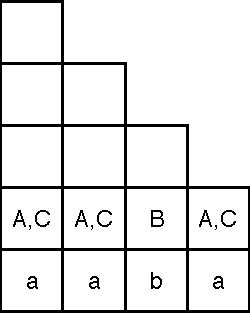
\includegraphics[width=0.22\textwidth]{img/CYKDemo1STEP1}
		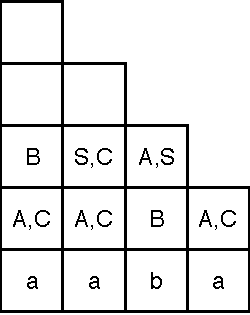
\includegraphics[width=0.22\textwidth]{img/CYKDemo1STEP2}
		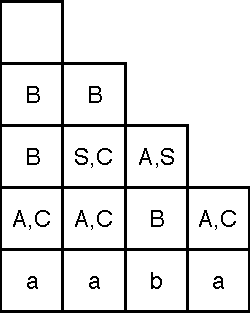
\includegraphics[width=0.22\textwidth]{img/CYKDemo1STEP3}
		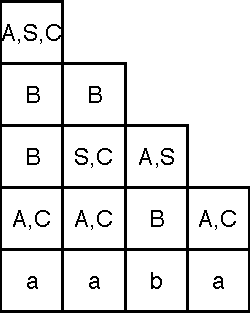
\includegraphics[width=0.22\textwidth]{img/CYKDemo1STEP4}
		\caption{Kroky \gls{gloss:CYK} algoritmu}
		\label{pic:cykSteps}
	\end{figure}
	
	Kód \ref{alg:cyk} poté slouží jako pseudokód \gls{gloss:CYK} algoritmu.
	
	\begin{listing}
		\begin{minted}[tabsize=3,escapeinside={(*}{*)}]{text}
pozice(řádek, sloupec):
	kombinace = vytvoř množinu
	počet_kombinací = délka slova - řádek
	pro v jdoucí do počet_kombinací:
		b_1 = bod(řádek + v + 1, sloupec)
		b_2 = bod(řádek + počet_kombinací - v, 
		          sloupec + počet_kombinací - v)
		kombinace.přidej((b_1, b_2))
	vrať kombinace
	
cyk(gramatika, slovo):
	pole = vytvoř dvojrozměrné pole veliksoti délky slova
	pro každý symbol slova:
		pravidla = najdi pravidla derivující se na symbol
		pole[délka slova][index] = pravidla.levá_strana	
	pro každý řádek i:
		pro každý sloupec j:
			pro každý prvek (b_1, b_2) v pozice(i, j):
				první_s = pole[b_1.x][b_1.y]
				druhý_s = pole[b_2.x][b_2.y]		
				pro každé pravidlo p_1:
					pokud p_1.pravá_strana = (první_s, druhý_s)
						pole[i][j] += p_1.levá_strana
	jestliže je gramatika.počáteční_symbol v pole[0][0]:
		úspěch
	jinak:
		neúspěch
		\end{minted}
		\caption{Pseudokód \gls{gloss:CYK} algoritmu}
		\label{alg:cyk}
	\end{listing}
	
	Pro samotnou konstrukci syntaktického stromu je potřeba algoritmus upravit. \gls{gloss:CYK} algoritmus během svého běhu nebude do tabulky ukládat neterminály, které se derivují na slovo, ale uloží si použité pravidlo a pozice symbolů pravé strany pravidla. Díky těmto informacím může algoritmus po úspěšném parsování sestavit syntaktický strom bez dodatečného procházení gramatiky nebo vstupního slova.
	
\include{analyzeAndDesign}

\chapter{Realizace}

	Následující kapitola se zabývá přípravou projektu, implementací, testováním a~nakonec publikováním knihovny. 
	Naší snahou v~této části práce je popsat fungování knihovny a~proces jejího vývoje. Algoritmy používané knihovnou jsou buď velmi jednoduché -- a tedy postačí jejich textový popis, nebo jsou již z~velké části popsány pseudokódem v~dřívějších kapitolách. Z~tohoto důvodu se budeme snažit minimalizovat ukázky zdrojového kódu za účelem přehlednosti a~konzistence práce. Kompletní zdrojový kód lze nalézt na přiloženém médiu či online na portálu GitHub \cite{GrammpyProject}.

	\section{Příprava prostředí}
		
		Vývojové prostředí a~metodika vývoje přímo ovlivňují, jakým způsobem software vzniká a~jakým způsobem mezi sebou vývojáři sdílejí změny.
		
		Prostředí jazyka Python bylo zvoleno poslední stabilní vydání, tedy verze \MathSymb{3.6.4}. Pod tímto prostředím je knihovna vyvíjena a~testována během vývoje, nicméně v~rámci \gls{gloss:CI} je knihovna otestována pod dalšími prostředími jazyka Python, a~to až do verze \MathSymb{3.3}, protože se jedná o~poslední podporovanou verzi v~Linuxové distribuci Fedora \cite{FedoraMultiplePythons}.
	
		Během vývoje knihovny bude použit nástroj \MathSymb{Git}. Jedná se o~nástroj široce používaný \cite{VersionControlSystem2016}
		a~většině vývojářů známý, který zároveň vyřeší požadavek \ref{req:codeVersioning}. V~souladu s~požadavky \ref{req:sourcesOnline} a~\ref{req:docOnline} budou zdrojové kódy umístěny veřejně na portálu \hyperlink{https://github.com/}{GitHub} \cite{GrammpyProject}, který je většině vývojářů taktéž známý.
		
		K~dodržení požadavku \ref{req:CI} byl zvolen nástroj \hyperlink{https://travis-ci.org/}{TraviCI} \cite{Travis}. Ten je pro otevřený software (open-source), kterým naše knihovna je, zcela zdarma. Konfigurace probíhá pouze jediným souborem \enquote{\MathSymb{.travis.yml}}. Tento nástroj spustí všechny testy nad knihovnou v~námi definovaných prostředích a~v~případě chyby tuto skutečnost nahlásí prostřednictvím e-mailu. TravisCI je taktéž integrován s~GitHubem, takže při libovolné změně zdrojového kódu jsou všechny testy spuštěny automaticky a~jejich výstup vložen na GitHub. čímž je splněn požadavek \ref{req:constistence}.
		
		V~případě verzování knihovny bylo zvoleno sekvenční verzování se třemi pozicemi \cite{semver}.
		\begin{itemize}
			\item Major -- \enquote{\textit{MAJOR version when you make incompatible API changes}} \cite{semver} -- major verse se mění při tzv. breaking changes, tedy při změnách, kvůli nimž nelze starý software, fungující se starou verzí knihovny, použít s~její verzí novou. Obecně je snahou měnit major verzi co nejméně, pokud možno vůbec. 
			\item Minor -- \enquote{\textit{MINOR version when you add functionality in a backwards-compatible manner}} \cite{semver} -- minor verze se mění se při vylepšení softwaru. Minor verze přinášejí uživatelům novou funkcionalitu, ale je dodrženo stejné rozhraní. Starý software tak může fungovat i~s~novější verzí knihov\-ny, než pro který byl napsán.
			\item Patch -- patche jsou změny knihovny za účelem opravy chyb. Na rozdíl od minor verze nepřináší novou funkcionalitu (eventuálně pouze minimální), ale spíše se soustřeďuje na opravu chyb resp. interní vylepšení knihovny.
		\end{itemize}
		Verze jsou psány za sebe a~odděleny tečkou -- \MathSymb{<major>.<minor>.<patch>} (například \MathSymb{1.2.0}).
		
		Dříve, než se pustíme do samotné implementace, ještě musíme zvolit název knihovny resp. jednotlivých modulů. Název je důležitý pro konečné publikování aplikace do online repositáře, ze kterého si knihovnu mohou stáhnout uživatelé. Pro základní modul reprezentující gramatiky byl zvolen název \MathSymb{grammpy}, pro jejich transformace modul \MathSymb{grammpy-transforms}. Modul obsahující jednotlivé parsery bude pojmenován \MathSymb{pyparsers}. Zdrojové kódy budou umístěny online a~to na portálu GitHub \cite{GrammpyProject}.
		
	\section{Reprezentace gramatik}
	
		Podoba modulu pro reprezentaci gramatik byla z~velké části již dána návrhem knihovny. Základem modulu je třída \Code{Grammar}, která gramatiku uchovává v~interních strukturách a~poskytuje ke gramatice rozhraní.
		
		Třída \Code{Grammar} byla implementována s~ohledem na zvolenou architekturu \MathSymb{Pipes and Filters}. Logika je rozdělena do několika vrstev, kde každá vrstva je reprezentována třídou.
		
		\begin{itemize}
			\item \Code{RawGrammar} -- poskytuje základní rozhraní pro manipulaci s~gramatikou. Poskytuje \gls{gloss:CRUD} operace pro terminály, neterminály, pravidla a~počáteční symbol. Provádí taktéž validaci parametrů, tedy že pravidlo dědí ze třídy \Code{Rule} a neterminál ze třídy \Code{Nonterminal}.
			\item \Code{StringGrammar} -- zpracovává vstupní parametry v~případě, kdy se jedná o~text. Text je v~Pythonu iterovatelný, tedy jde s~ním zacházet jako s~polem. To je nežádoucí, protože u pole očekáváme jeho projití a~přidání všech prvků v~poli, zatímco text považujeme za dále nedělitelný. Třída \Code{StringGrammar} se stará o~to, že text nebude brán jako pole.
			\item \Code{MultipleRulesGrammar} -- z~návrhu knihovny lze vytvořit třídu reprezentující několik pravidel současně. To je komplikace při vnitřní reprezentaci, protože následně můžeme chtít odstranit pouze jedno z~pravidel. Třída \Code{MultipleRulesGrammar} tyto pravidla rozdělí do samostatných tříd, které následně vloží do gramatiky. Díky této logice lze s~pravidly manipulovat jednotlivě.
			\item \Code{PrettyApiGrammar} -- rozšiřuje rozhraní knihovny o~některé metody, které jsou založeny nad standardním rozhraním. Jedná se především o~zkrácení zápisu a~eventuálně standardizaci parametrů.
			\item \Code{RulesRemovingGrammar} -- je-li z~gramatiky odstraněn neterminál nebo terminál, očekávali bychom také odstranění všech pravidel, které tento terminál resp. neterminál obsahují. Třída \Code{RulesRemovingGrammar} obstarává tuto logiku.
			\item \Code{CopyableGrammar} -- tato třída obstarává implementaci kopírování, tedy hluboké kopie (deep copy) a mělké kopie (shallow copy).
			\item \Code{Grammar} -- jedná se o~zastřešující třídu, která skrývá vnitřní implementaci. Budou--li výše zmíněné třídy gramatiky změněny nebo přepsány, jejich skrytím za třídu \Code{Grammar} je zajištěna kompatibilita se~starými aplikacemi (za předpokladu, že se nezmění rozhraní).
		\end{itemize}
	
		Stejný přístup byl zvolen i~pro třídu \Code{Rule} reprezentující pravidlo.
		
		\begin{itemize}
			\item \Code{BaseRule} -- tato třída obsahuje základ pravidel. Má nadefinované statické vlastnosti a~logiku s~dopočítáváním zbylých vlastností (viz kapitola \ref{sec:designOfLibrary}). Třída dále obsahuje definici hashovací funkce a porovnávacího operátoru.
			\item \Code{ValidationRule} -- třída \Code{ValidationRule} obsahuje logiku související s~validací pravidel. Tato logika se volá ve chvíli, kdy je pravidlo vkládáno do gramatiky. Kontroluje se tak, že jsou pravidla nadefinována syntakticky správně, ale také že všechny symboly použité v~pravidlu jsou v~gramatice k~dispozici.
			\item \Code{InstantiableRule} -- jak bylo řečeno v~sekci návrhu, pravidla se budou instanciovat a~budou sloužit jako entita v~\gls{gloss:AST}. Tato třída definuje potřebné atributy a~metody potřebné k~tomuto účelu.
			\item \Code{Rule} -- stejně jako třída \Code{Grammar}, je třída \Code{Rule} pouze abstrakcí, která odděluje vnitřní implementaci od jejího použití. 
		\end{itemize}
	
		Modul kromě výše zmíněných tříd obsahuje ještě třídy další. Některé ze tříd jsou pomocné a~jsou určeny pouze k~interním účelům modulu. Tyto třídy nejsou exportovány ven z~modulu a~pro uživatele knihovny se jeví jako nedostupné.
		
		\begin{itemize}
			\item \Code{RuleConnectable} -- je rozhraní umožňující propojit entity pomocí pravidel. 
			\item \Code{Terminal} -- je třída reprezentující terminál v~\gls{gloss:AST}, resp. u~operací s~terminály pracujících. Třída dědí ze třídy \Code{RuleConnectable} a~v~aktuální implementaci poskytuje jen metodu \Code{symbol}, která vrátí skutečný symbol do gramatiky vložený.
			\item \Code{Nonterminal} -- třída \Code{Nonterminal} neposkytuje žádnou implementaci, pouze dědí ze třídy \Code{RuleConnectable}. Tato třída slouží jako bázová třída pro ostatní neterminály, které jsou identifikovány právě dědičností z~této třídy.
			\item \Code{WeakList} -- je interní třída představující pole se slabými (\MathSymb{weak}) odkazy. Python používá pro uvolnění paměti garbage collector (\gls{gloss:GC}), který používá tzv. reference counting. Ten je náchylný na odkazovací smyčky, které se v~programu vyskytují (pravidlo má odkaz na symbol a~symbol má odkaz zpět na pravidlo). Použitým slabých odkazů se tento problém eliminuje. \Code{WeakList} je použit interně v~implementaci třídy \Code{InstantiableRule}.
			\item \Code{HashContainer} -- tato třída slouží jako jednoduchá množina, založená na hash hodnotách. Na rozdíl od výchozí implementace množiny (která je taktéž založená na hash hodnotách) má \Code{HashContainer} změněné rozhraní. Použita je pro uchovávání terminálů, neterminálů a~pravidel ve třídě \Code{RawRule}.
		\end{itemize}
	
		Nakonec má modul nadefinovanou hierarchii výjimek. Všechny výjimky dědí ze třídy \Code{GrammpyException}, která sama dědí ze třídy \mintinline{c}{Exception}. Kompletní hierarchie je zachycena na obrázku \ref{fig:grammpyExceptions}.
		\begin{itemize}
			\item \Code{GrammpyException} -- základní, společná třída.
			\item \Code{CannotConvertException} -- konverze neproběhla v~pořádku, dědí také z~\Code{ValueError}.
			\item \Code{NotASingleSymbolException} -- na místě, kde má být jeden symbol, je jich uvedeno více.
			\item \Code{NotRuleException} -- parametr není pravidlo, mimo \Code{GrammpyException} dědí také z~\Code{TypeError}.
			\item \Code{NotNonterminalException} -- parametrem není neterminál, dědí také z~\Code{TypeError}.
			\item \Code{RuleException} -- pravidlo je nadefinováno syntakticky nesprávně nebo nevalidně, kromě \Code{GrammpyException} dědí také ze třídy \Code{ValueError}.
			\item \Code{RuleSyntaxException} -- špatná syntaxe pravidla.
			\item \Code{TerminalDoesNotExistsException} -- použitý terminál v~gramatice neexistuje.
			\item \Code{NonterminalDoesNotExistsException} -- použitý neterminál v gramatice neexistuje.
			\item \Code{UselessEpsilonException} --	\EpsS symbol je špatně použit.
			\item \Code{CantCreateSingleRuleException} -- rozdělení na jednotlivé pravidla skončilo chybou.
			\item \Code{RuleNotDefinedException} -- pravidlo není nadefinováno.
			\item \Code{TreeDeletedException} -- odkazovaný element \gls{gloss:AST} byl již smazán.
		\end{itemize}
	
		Výsledek implementace je znázorněn v~diagramu na obrázku \ref{fig:grammpyClasses}, resp. na obrázku \ref{fig:grammpyExceptions}, kde je znázorněna hierarchie výjimek. 
		
	\section{Transformace a~parsování}
	
		Algoritmy pro transformaci jsou pouze implementací pseudokódů, které byly ukázány v~kapitole o~operacích s~gramatikami. Z~tohoto důvodu bude kód jednotlivých algoritmů vynechán. Kompletní implementace je k~dispozici na přiloženém mediu nebo online \cite{GrammpyProject}.
		
		Každý z~algoritmů zpravidla definuje vlastní neterminály resp. pravidla, kterými nahradí modifikovaný neterminál resp. pravidlo. Díky jejich typu lze poté provést zpětnou transformaci \gls{gloss:AST}. Dále následuje popis algoritmů, které jsou v~knihovně implementovány, zároveň s~jejich typy.
		
		\begin{itemize}
			\item \Code{remove_nongenerating_nonterminals} -- odstraní negenerující neterminály z~gramatiky. Algoritmus nedefinuje žádné vlastní třídy, protože se jedná pouze o~optimalizační techniku.
			
			\item \Code{remove_unreachable_symbols} -- odstraní nedostupné symboly. Opět se jedná pouze o~optimalizační techniku, a~tak algoritmus nedefinuje vlastní třídy.
			
			\item \Code{remove_rules_with_epsilon} -- odstraní \EpsS pravidel. Algoritmus definuje vlastní třídu pro pravidlo -- \Code{EpsilonRemovedRule}. V této třídě je uloženo, ve kterém pravidle byl symbol přepsán na \EpsS, jeho pozici a~dále sekvence pravidel, které k~\EpsS symbolu vedly.
			
			Algoritmus pro zpětnou transformaci na místě, kde je pravidlo typu \Code{EpsilonRemovedRule} použito, vytvoří původní pravidlo. Poté vytvoří sekvenci pravidel, která vedla k~\Eps~symbolu, a~vloží ji na pozici určenou indexem.
			
			\item \Code{remove_unit_rules} -- odstraní jednoduché pravidla z~gramatiky. Algoritmus definuje pravidlo \Code{ReducedUnitRule}, které nahradí pravidla, na jejichž pravé straně se vyskytuje symbol vedoucí k~jednoduchému pravidlu. Třída \Code{ReducedUnitRule} si podobně jako \Code{EpsilonRemovedRule} ukládá, ze kterého pravidla vznikla a~sekvenci jednoduchých pravidel, které k~transformaci vedly.
			
			Algoritmus pro zpětnou transformaci probíhá taktéž obdobně -- nejdříve je vytvořena sekvence jednoduchých pravidel, poté konečné pravidlo a~tato struktura je vložena na patřičné místo v~\gls{gloss:AST}.
			
			\item \Code{transform_to_chomsky_normal_form} -- transformuje gramatiku do \gls{gloss:CNF}. Tento algoritmus definuje několik tříd, některé z~nich pro interní potřeby. Neterminály definuje tři:
			\begin{itemize}
				\item \Code{ChomskyNonterminal} -- bázová třída pro zbylé dva neterminály,
				\item \Code{ChomskyGroupNonterminal} -- představuje neterminál reprezentující více neterminálů,
				\item \Code{ChomskyTermNonterminal} -- představuje neterminál přímo derivovatelný na terminál.
			\end{itemize}
		
			K~těmto neterminálům algoritmus definuje i~patřičná pravidla.
			\begin{itemize}
				\item \Code{ChomskyRule} -- bázová třída pro zbylé pravidla.
				\item \Code{ChomskySplitRule} -- pravidlo vzniklé rozdělením pravidla do dvou neterminálů. Druhým symbolem pravé strany pravidla je vždy pravidlo \Code{ChomskyGroupNonterminal}, který reprezentuje všechny symboly pravé strany s~výjimkou prvního.
				\item \Code{ChomskyRestRule} -- reprezentuje zbylou část pravidla neterminálu \Code{ChomskyGroupNonterminal}. Jedná se pouze o~dočasný objekt, protože v~další iteraci je i~toto pravidlo rozděleno na dva neterminály -- vznikne z~něj tedy opět pravidlo typu \Code{ChomskySplitRule}.
				\item \Code{ChomskyTerminalReplaceRule} -- slouží jako náhrada pravidla na jehož pravé straně jsou dva symboly, ale jeden z~nich je terminál. Tento symbol je nahrazen \Code{ChomskyTermNonterminal} a~dále je přidáno pravidlo typu \Code{ChomskyTermRule}.
				\item \Code{ChomskyTermRule} -- je pravidlo, které přímo derivuje neterminál na terminál.
			\end{itemize}
		
			Každý z~definovaných neterminálů resp. terminálů definují atributy, na jejichž základě lze transformovat \gls{gloss:AST}.
		\end{itemize}
	
		Modul kromě toho definuje pomocné třídy \Code{Manipulations} a \Code{Traversing}, které zjednodušují práci s~\gls{gloss:AST}. Třída \Code{Manipulations} poskytuje rozhraní pro nahrazení pravidla v~\gls{gloss:AST} jiným pravidlem, resp. nahrazení terminálu či neterminálu jiným symbolem. Třída \Code{Traversing} dále definuje metody pro procházení \gls{gloss:AST}. V~základu implementuje procházení metodou pre-order a~post\=/or\-der, ale také abstraktnější verzi pro procházení na základě callbacku.
		
		Kompletní návrh modulu lze nalézt na obrázku \ref{fig:grammpyTransformsClasses}. Použitá pravidla jsou poté na obrázku \ref{fig:grammpyTransformsRules} a~neterminály na obrázku \ref{fig:grammpyTransformsNonterminals}.
		
		\vspace{1em}
		
		Modul \MathSymb{pyparsers} se skládá pouze z~jedné funkce -- \Code{cyk}. Tato funkce provede \gls{gloss:CYK} algoritmus a~navrátí \gls{gloss:AST}. Modul obsahuje další pomocné třídy, které jsou interně použity při algoritmu.
		\begin{itemize}
			\item \Code{Point} -- reprezentuje bod o~souřadnicích \MathSymb{x} a \MathSymb{y}. Interně se nejedná o~třídu, ale o~tzv. namedtuple \cite{namedtuple}.
			\item \Code{Field} -- reprezentuje pyramidovou strukturu, nad kterou operuje \gls{gloss:CYK} algoritmus.
			\item \Code{PlaceItem} -- zastřešuje strukturu uchovávající použité pravidlo a~jeho potomky.
		\end{itemize}
	
		Algoritmus si nejprve vytvoří instanci typu \Code{Field}. Poté si vytvoří dva překladové slovníky -- jeden pro pravidla, která se přímo derivují na neterminály, a druhý, jehož klíčem jsou dva neterminály a~hodnotou je vždy pravidlo na tyto neterminály přímo derivovatelné. Na základě prvního slovníku jsou poté nalezeny neterminály, které se přímo derivují na vstupní terminály, a~tyto neterminály jsou vyplněny do posledního řádku tabulky. Algoritmus dále probíhá stejně, jak je to uvedeno v~jeho pseudokódu.
		
		Po dokončení algoritmus zkontroluje, zda je počáteční symbol v~prvním řádku pole (viz obrázek \ref{pic:cykSteps}) a~pokud ne, vyvolá výjimku. V~případě, kdy se počáteční symbol v~prvním řádku tabulky vyskytuje, algoritmus pokračuje s~tvorbou \gls{gloss:AST}. Díky struktuře \Code{PlaceItem}, ve které si algoritmus ukládá použitá pravidla, lze \gls{gloss:AST} vytvořit bez dalšího procházení vstupního slova nebo gramatiky. Zdrojové kódy jsou opět na přiloženém mediu a~online.
	
		Vzhledem k~tomu, že rozhraním modulu je pouze jedna funkce, není zde k~tomuto modulu zobrazen diagram.
		
	\section{Testování}	
		Pro otestování knihovny byl zvolen framework \Code{unittest}. Tento framework je dostupný jako Python modul přímo ve výchozí instalaci, není tedy třeba instalovat knihovny třetích stran. Jedná se o~testovací framework určený především k~jednotkovým testům (unit testům). Vzhledem k~faktu, že implementujeme pouze knihovnu a~nikoliv celou aplikaci, je jednotkové (resp. integrační) testování dostatečným ověřením jejího správného fungování. Systémové či uživatelské testy vzhledem k~povaze problému ani nelze provádět. Knihovna je otestována více než 450 jednotkovými testy.
		
		Pokrytí kódu (anglicky code coverage) \cite{Ammann:2008:IST:1355340} je analytický přístup ověřující, že všechen kód, ze kterého se software skládá, byl alespoň jednou spuštěn.
		Při vysokém pokrytí kódu máme jistotu, že téměř celá aplikace byla spuštěna a~v~rámci tohoto běhu funguje jak má. Vysoké pokrytí nám nicméně nezaručuje, že software funguje správně, protože mohou nastat situace, se kterými není v~kódu počítáno.
		Nástroje určující pokrytí kódu detekují, že byl kód spuštěn, ale samotnou chybu neobjeví. Software, jenž obsahuje grafické rozhraní, je zpravidla pokryt hůře, protože testování grafického prostředí je náročné a~vyžaduje speciální nástroje. V~našem případě můžeme zvolit požadované pokrytí větší (viz požadavek \ref{req:coverage}), protože se jedná pouze o~knihovnu, kterou lze v~běžných případech otestovat téměř celou \cite{Ammann:2008:IST:1355340}. Během vývoje se stav pokrytí neustále mění v~závislosti na fázi vývoje a~vydání. Knihovna se nicméně řídí požadavkem \ref{req:coverage} a~její pokrytí neklesá pod 90 \%. Publikované verze knihovny mají zpravidla pokrytí kódu větší, tradičně 100 \%.
		
		Jako nástroj měřící pokrytí kódu byl zvolen framework (resp. modul) \hyperlink{https://coverage.readthedocs.io/en/coverage-4.5.1/}{Coverage.py} \cite{coveragePy}, který je napsán v~jazyce Python, a pro své fungování vyžaduje pouze instalaci tohoto modulu. Pokrytí kódu je automaticky generováno na základě jednotkových testů. Data jsou poté přenesena do nástroje \hyperlink{https://coveralls.io/}{Coveralls} \cite{coveralls}, který podle dodaných dat generuje přehledné reporty. Ty obsahují celkové pokrytí kódu, pokrytí jednotlivých tříd resp. souborů a~samozřejmě také změnu pokrytí mezi jednotlivými verzemi softwaru. Nástroj je opět pro otevřený software zdarma a~díky integraci s~nástroji GitHub a~TravisCI jsou reporty generovány pro každou verzi softwaru automaticky.
		
		
		

\chapter{Demonstrace knihovny na příkladech}

	V~následující kapitole je knihovna použita pro parsování aritmetických výrazů, regulárních výrazů a~lambda kalkulu. Základ aplikace a~postupy zůstávají stále podobné prvnímu příkladu. Z~tohoto důvodu budou pro jednotlivé příklady ukázány pouze klíčové části programu. Kompletní zdrojové kódy jsou na přiloženém mediu.
	
	\section{Parser aritmetických výrazů}
	
		Nyní již máme všechny prostředky potřebné pro tvorbu parseru. V~této sekci budeme demonstrovat fungování programu na parseru aritmetických výrazů, tedy výrazů podporujících operace $+,-,*,/$ a použití závorek.
		
		Budeme vycházet z~gramatiky \GrammarDef\space kde
		
		\begin{tabular}{rl}
			$N=$ & $\left\{ Number, MultipleDivide, PlusMinus \right\}$\\
			$T=$ & $\left\{0,1,2,3,4,5,6,7,8,9,+,-,*,/,\left(,\right)\right\}$\\
			$S=$ & $PlusMinus$\\
			$R=$ & $\left\{ \Rule{Number}{0},\Rule{Number}{1},\cdots,\Rule{Number}{9}, \right.$ \\
			& $\Rule{Number}{Number 0},\cdots,\Rule{Number}{Number 9},$ \\
			& $\Rule{PlusMinus}{PlusMinus + MultipleDivide},$ \\
			& $\Rule{PlusMinus}{PlusMinus - MultipleDivide},$ \\
			& $\Rule{PlusMinus}{MultipleDivide},$ \\
			& $\Rule{MultipleDivide}{MultipleDivide * Number},$ \\
			& $\Rule{MultipleDivide}{MultipleDivide / Number},$ \\
			& $\Rule{MultipleDivide}{Number},$ \\
			& $\Rule{Number}{\left(\right. PlusMinus \left.\right)}$ \\
		\end{tabular}
		
		Nejdříve nadefinujeme neterminál, který bude mít jeden atribut -- vytvoříme tak atributovanou gramatiku (kód \ref{alg:calcAttributedNonterminal}). Z~toho neterminálu budou dědit zbývající neterminály.
		
		\begin{listing}
			\begin{minted}[tabsize=3]{python}
class Common(Nonterminal):
	def __init__(self):
		self._attribute = None
	
	@property
	def attribute(self):
		if self._attribute is None:
			self.to_rule.compute()
		return self._attribute
	
	@attribute.setter
	def attribute(self, value):
		self._attribute = value
			\end{minted}
			\caption{Definice atributovaného neterminálu}
			\label{alg:calcAttributedNonterminal}
		\end{listing}
		
		Jak je v~kódu vidět, atribut se počítá až ve chvíli, kdy je o~něj požádáno (tzv. lazy evaluzation). Přitom se zavolá metoda \Code{compute} na pravidlu, které neterminál přepisuje. V~tomto případě jsou totiž všechny atributy syntetizované. Nyní nadefinujeme pravidla a jejich sémantiku. Vzhledem k~množství pravidel je nebudeme vypisovat všechny, ale jako příklad uvedeme pouze $\Rule{MultipleDivide}{MultipleDivide / Number}$.
		
		\begin{listing}
			\begin{minted}[breaklines,tabsize=3]{python}
class DivideApplied(Rule):
	fromSymbol = MultipleDivide
	right = [MultipleDivide, DivideOperator, Number]
	
	def compute(self):
		parent = self.from_symbols[0]
		left_child = self.to_symbols[0]
		right_child = self.to_symbols[2]
		result = left_child.attribute / right_child.attribute
		parent.attribute = result
			\end{minted}
			\caption{Pravidlo $\Rule{MultipleDivide}{MultipleDivide / Number}$}
			\label{alg:calcMultipleDivide}
		\end{listing}
		
		Na základě terminálů, neterminálů a~pravidel poté můžeme nadefinovat gramatiku (algoritmus \ref{alg:calcGrammarDefinition}).
		
		\begin{listing}
			\begin{minted}[breaklines,tabsize=3]{python}
g = Grammar(terminals=[0, 1, 2, 3, 4, 5, 6, 7, 8, 9,PlusOperator, MinusOperator, MultipleOperator,DivideOperator,LeftBracket, RightBracket],
	nonterminals=[Number, MultipleDivide, PlusMinus],
	rules=[NumberDirect, NumberCompute,DivideApplied, MultipleApplied, NoDivideMultiple, MinusApplied, PlusApplied, NoPlusMinus, BracketsApplied],
	start_symbol=PlusMinus)
			\end{minted}
			\caption{Definice aritmetické gramatiky}
			\label{alg:calcGrammarDefinition}
		\end{listing}
		
		Nyní použijeme gramatiku ke zpracování výrazu $10 + ( 5 * 2 + 4 ) / 2 * 4$. V~rámci tohoto příkladu není vytvořen lexikální analyzátor, proto nebude vstupní slovo parsováno z~příkazové řádky, ale bude zapsáno přímo v~programu. Před samotným parsování ještě musíme provést transformace gramatiky do \gls{gloss:CNF} a~po parsování provést zpětnou transformaci \gls{gloss:AST} (algoritmus \ref{alg:calcParsing}).
		
		\begin{listing}
			\begin{minted}[breaklines,tabsize=3]{python}
ContextFree.remove_useless_symbols(g, transform_grammar=True)
ContextFree.remove_rules_with_epsilon(g, transform_grammar=True)
ContextFree.remove_unit_rules(g, transform_grammar=True)
ContextFree.remove_useless_symbols(g, transform_grammar=True)
ContextFree.transform_to_chomsky_normal_form(g, transform_grammar=True)

parsed = cyk(g, [1, 0, PlusOperator, LeftBracket, 5, MultipleOperator, 2, PlusOperator, 4, RightBracket, DivideOperator, 2, MultipleOperator, 4])

parsed = InverseContextFree.transform_from_chomsky_normal_form(parsed)
parsed = InverseContextFree.unit_rules_restore(parsed)
parsed = InverseContextFree.epsilon_rules_restore(parsed)
parsed = InverseCommon.splitted_rules(parsed)
print(parsed.attribute)
			\end{minted}
			\caption{Proces parsování aritmetických výrazů}
			\label{alg:calcParsing}
		\end{listing}
	

	\section{Parser regulárních výrazů}
		
		Obecný parser regulárních výrazů má široké uplatnění. Asi nejevidentnější je převod regulárního výrazu do stavového automatu. Stavovým automatem lze poté testovat, zda vstupní slovo vyhovuje nebo nevyhovuje regulárnímu výrazu.
		
		V~tomto příkladě budeme nicméně demonstrovat přesně opačné použití -- vypsání všech slov (s~jistými omezujícími podmínkami), které zadanému regulárnímu výrazu vyhovují. Takový program lze využít například pro prolamování hesel, která mají předem daný formát.
		
		Při formátu regulárních výrazů vycházíme ze zdroje \cite{Aho:1986:CPT:6448}. Program je založen na gramatice \GrammarDef.
		
		\begin{tabular}{rl}
			$N=$ & $\left\{ Symb, Concat, Iterate, Or\right\}$\\
			$T=$ & $\left\{ a,b,c,\cdots,y,z,+,*,\left(\right.,\left.\right) \right\}$\\
			$S=$ & $Or$\\
			$R=$ & $\left\{\right.  \Rule{Or}{Or + Or}, \Rule{Or}{Concat}, $ \\
			& $\Rule{Concat}{Iterate Concat}, \Rule{Concat}{Iterate},$ \\
			& $\Rule{Iterate}{{Symb}^{\ast}}, \Rule{Iterate}{Symb}$ \\
			& $\Rule{Symb}{\left(\right. Or \left.\right)},$ \\
			& $\Rule{Symb}{a}, \Rule{Symb}{b}, \cdots, \Rule{Symb}{z} \left.\right\}$ \\
		\end{tabular}
		
		Na rozdíl od předchozího příkladu nyní ukážeme přístup, kdy nebude sémantika aplikace uložena v~pravidlech, ale přímo v~neterminálech. Každý z~neterminálů bude mít metodu \Code{get}, která vrátí seznam slov, které danému regulárnímu podvýrazu vyhovují. Například pro neterminál \MathSymb{Symb} který by měl pouze pravidlo $\Rule{Symb}{a}$ by byla metoda implementována pouze jako navrácení hodnoty terminálu \Code{return [self.to_rule.to_symbols[0].s]}.
		Pro představu ukážeme metodu \Code{get} neterminálu \MathSymb{Concat} (algoritmus \ref{alg:concatNonterminal}).
		
		\begin{listing}
			\begin{minted}[tabsize=3]{python}
class Concat(Nonterminal):
	def get(self, i, f):
		if len(self.to_rule.to_symbols) == 1:
			return self.to_rule.to_symbols[0].get(i, f)
		new = []
		left = self.to_rule.to_symbols[0].get(i, f)
		right = self.to_rule.to_symbols[1].get(i, f)
		for l in left:
			for r in right:
				new.append(l + r)
		return new
			\end{minted}
			\caption{Implementace metody \Code{get} neterminálu \MathSymb{Concat}}
			\label{alg:concatNonterminal}
		\end{listing}
		
		Parametry \Code{i} a \Code{f} udávají maximální počet iterací, resp. znaky vyplnění na místě, kde má iterace skončit. Tyto parametry jsou relevantní pouze pro neterminál \MathSymb{Iterate}. Jsou využity k~omezení délky slova, například pro regulární výraz \enquote{ab*(def+xy*z)} se jako nejdelší slovo vygeneruje \enquote{abb...bbxyy...yyz}, je--li $i=3$ a $f=\cdots$.
		
		Běh aplikace je ukázán na obrázku \ref{pic:runRegexInverse}.
		
		\begin{figure}
			\begin{minted}[tabsize=3]{bash}
$ python3 run.py -i 2 -f "___" "(a+b)*c"
c
ac
aac
a___ac
c
bc
bbc
b___bc
			\end{minted}
			\caption{Ukázka běhu parseru regulárních výrazů}
			\label{pic:runRegexInverse}
		\end{figure}
	
	\section{Interpret lambda kalkulu}
	
		V~tomto příkladě budeme tvořit interpret lambda kalkulu. Při definici lambda kalkulu vycházíme ze zdroje \cite{hindley1986introduction}. Na rozdíl od předchozích příkladů, které se zaměřovaly čistě na parsování, musíme u~interpretu lambda kalkulu řešit implementaci interpretu. 
		
		Jedním z~problémů je zjednodušení vstupního textu. Ačkoliv by bylo možné parsovat vstup v~jeho textové podobě, velmi by se tím komplikovala gramatika. Pro příklad uveďme bílé znaky, které nemají ze sémantického hlediska žádný význam. Také identifikátory mohou nabývat téměř nekonečného počtu hodnot, ale tyto hodnoty jsou z~hlediska parsovacího procesu nepodstatné. V~aplikaci proto před samotným parsováním použijeme lexikální analyzátor, který převede vstupní text do série tokenů, které teprve budou zpracovány samotným parserem. Budeme tím demonstrovat použití lexikálního analyzátoru ve spojení s~vytvořenou knihovnou
		
		Dalším z~problémů je samotná interpretace. Aplikace musí nejenom naparsovat vstup, ale i~správně provádět operace lambda kalkulu (konkrétně $\alpha$ redukci, $\beta$ redukci a další). Jelikož zmíněné operace nijak nesouvisejí s~procesem parsování ani s~touto prací, bude použita existující knihovna.
		
		Samotná aplikace bude rozdělena do několika částí.
		\begin{itemize}
			\item Syntaktický analyzátor -- jedná se o~podprogram převádějící vstupní text na sérii tokenů. Gramatika je nadefinována nad těmito tokeny a~nikoliv nad samotným vstupním textem.
			\item Parser -- hlavní část programu z~hlediska této práce. Parser převede vstupní sérii tokenů na \gls{gloss:AST}.
			\item Reprezentace -- \gls{gloss:AST} je převeden do struktur vyžadovaných knihovnou pro interpretaci lambda kalkulu.
			\item Interpretace -- reprezentace je intepretována a~výstup je zobrazen uživateli.
		\end{itemize}
	
		Sémantická analýza je vyřešena knihovnou \MathSymb{PLY} (Python Lex--Yacc) \cite{PLY}. Jak název napovídá, knihovna je velmi silně ovlivněna nástroji \MathSymb{Lex} a \MathSymb{Yacc}. Jejím účelem je spojení těchto nástrojů a~jejich implementace v~jazyce Python. Z~knihovny byl použit pouze modul \Code{lex}, tedy modul zprostředkovávající lexikální analýzu. Syntaxe je velmi podobná syntaxi klasického nástroje \MathSymb{Lex}, pouze s~tím rozdílem, že je celý proces definován v~nativním Pythonu. Pro ukázku uveďme vytvoření tokenu představující proměnnou (algoritmus \ref{alg:lexVariable}), která může nabývat libovolné kombinace velkých písmen, malých písmen a~jednoduchých uvozovek.
		
		\begin{listing}
			\begin{minted}[tabsize=3]{python}
def t_VARIABLE(t):
	r'[a-zA-Z\']+'
	t.value = Variable(t.value)
	return t
			\end{minted}
			\caption{Generování tokenu symbolizující proměnnou}
			\label{alg:lexVariable}
		\end{listing}
	
		Parsování probíhá podobně, jako je tomu v~předchozích případech, až na rozdíl identifikace terminálů. Jak bylo řečeno, knihovna terminály porovnává podle jejich hash hodnoty. Budou-li dva objekty mít stejnou hash, budou interpretovány jako ekvivalentní. V~našem případě bude hash instance vracet hash třídy -- díky tomu lze instanci s~libovolnou hodnotou interpretovat jako terminál určité třídy. Ukážeme to na příkladu terminálu reprezentujícím číslo (algoritmus \ref{alg:termNumber}). Ačkoliv bude na vstupu několika terminálů, každý s~jiným atributem \Code{value}, parsovací algoritmus je bude považovat za ekvivalentní a~použije adekvátní pravidla.
	
		\begin{listing}
			\begin{minted}[tabsize=3]{python}
class Number:
	def __init__(self, value):
		self.value = value
	def __hash__(self):
		return hash(Number)
			\end{minted}
			\caption{Terminál reprezentující číslo}
			\label{alg:termNumber}
		\end{listing}
	
		Samotná gramatika \GrammarDef\space popisující lambda kalkul je k~prohlédnutí níže.
	
		\begin{tabular}[ht!]{rl}
			$N=$ & $\left\{\right. Nobracketexpression, Expression, Expressionbody,$ \\
				 & $Lambda, Parameters \left.\right\}$ \\
			$T=$ & $\left\{\right. Lambdakeyword, Dot, Leftbracket, Rightbracket,$ \\
			     & $Number, Variable, Parameter \left.\right\}$ \\	
			$S=$ & $Nobracketexpression$ \\
			$R=$ & $\left\{\right.  \Rule{Nobracketexpression}{Expressionbody},$ \\
			& $\Rule{Expressionbody}{Variable Expressionbody},$ \\
			& $\Rule{Expressionbody}{Variable},$ \\
			& $\Rule{Expressionbody}{Number Expressionbody},$ \\
			& $\Rule{Expressionbody}{Number},$ \\
			& $\Rule{Expressionbody}{Lambda Expressionbody},$ \\
			& $\Rule{Expressionbody}{Lambda},$ \\
			& $\Rule{Expressionbody}{Expression Expressionbody},$ \\
			& $\Rule{Expressionbody}{Expression},$ \\
			& $\Rule{Expression}{Leftbracket Nobracketexpression Rightbracket}$\\
			& $\Rule{Lambda}{Leftbracket Lambdakeyword Parameters}, $ \\
			& $Dot Nobracketexpression Rightbracket,$ \\
			& $\Rule{Parameters}{\varepsilon},$ \\
			& $\Rule{Parameters}{Parameter Parameters},$ \\
			& $\Rule{Parameters}{Parameter}  \left.\right\}$ \\
		\end{tabular}
	
		Sémantická část gramatiky je tentokrát smíšená -- některá sémantická pravidla jsou definována na pravidlech, některá na neterminálech. Protože se jedná pouze o~demonstraci knihovny, nebude implementace detailněji popsána. V~případě zájmu jsou zdrojové kódy na přiloženém mediu.
		
		Pro samotnou reprezentaci a~interpretaci knihovny byla zvolena knihovna \MathSymb{lambda{\_}interpreter} \cite{lambdaInterpreter}. Tato knihovna vznikla jako semestrální práce v~předmětu \enquote{Programovací paradigmata} (BI--PPA) studentkou Simonou Kurňavovou na \gls{gloss:FIT} \gls{gloss:CVUT}. 
		Tato knihovna definuje vlastní struktury pro definici výrazů v~lambda kalkulu. Sémantická část gramatiky spočívá právě v~převodu \gls{gloss:AST} do struktur vyžadovaných knihovnou \MathSymb{lambda{\_}interpreter}.
		
		Ná závěr je na reprezentaci opakovaně aplikována $\beta$ redukce a~mezivýsledky jsou zobrazeny uživateli. Běh programu lze vidět na obrázku \ref{pic:lambdaInterpreterRun}.
		
		\begin{figure}
			\begin{minted}{text}
>>>((lambda x. ((lambda y. (y x)) x y)) z)
((lambda x. ((lambda y. (y x)) x y)) z)
((lambda y. (y z)) z y)
((z z) y)
>>>((lambda var y. ((lambda z. ((lambda f. (z f)) z)) var)) 3 7)
((lambda var y. ((lambda z. ((lambda f. (z f)) z)) var)) 3 7)
((lambda y. ((lambda z. ((lambda f. (z f)) z)) 3)) 7)
((lambda z. ((lambda f. (z f)) z)) 3)
((lambda f. (3 f)) 3)
(3 3)
>>>(lambda x (y). x y)
Invalid input
>>>
			\end{minted}
			\caption{Ukázka běhu interpretu lambda kalkulu}
			\label{pic:lambdaInterpreterRun}
		\end{figure}
		
		
	
	

\begin{conclusion}
	Cílem práce bylo navrhnout, implementovat a~otestovat knihovnu, která je schopná na základě dodané gramatiky parsovat vstup.
	
	Funkcionalita byla patřičně navržena, implementována, otestována a~publikována v~knihovně \MathSymb{grammpy} \cite{GrammpyProject}. Knihovna přitom splňuje všechny požadavky, které na ni byly kladeny. Správné fungování knihovny je ověřeno více než 450 testy, které pokrývají téměř 100 \% kódu knihovny.
	V~práci bylo fungování knihovny demonstrováno na třech příkladech -- parser aritmetických výrazů, parser regulárních výrazů a~interpret lambda kalkulu.
	
	Knihovna v~aktuální implementaci poskytuje rozhraní nutné ke správnému fungování. Jedná se o~základní verzi, sloužící primárně k~ověření správného návrhu a~sběru zpětné vazby pro budoucí vývoj. Knihovna má stále několik oblastí, které lze dále rozvíjet -- implementace dalších parsovacích algoritmů nebo rozšíření rozhraní. Je v~plánu knihovnu dále rozvíjet i~po odevzdání této práce.
	
	Celkově hodnotíme výsledek práce pozitivně. Knihovna splňuje všech\-ny požadavky, které od ní byly očekávány. Během práce na tomto projektu již bylo nad knihovnou postaveno několik aplikací, které byly zmíněny v~poslední kapitole.
	Tyto aplikace jednak demonstrují fungování knihovny, ale také mají jasný účel a~dokážeme si představit jejich použití i~mimo kontext této práce.
\end{conclusion}

\bibliographystyle{csn690}
\bibliography{bibliography}

%\cleardoublepage
%\listoflistings
%\addcontentsline{toc}{chapter}{Seznam algoritmů}

%\cleardoublepage
%\listoffigures

\appendix

\cleardoublepage
\chapter{Obrazová příloha}
	\begin{figure}				
		\centering
		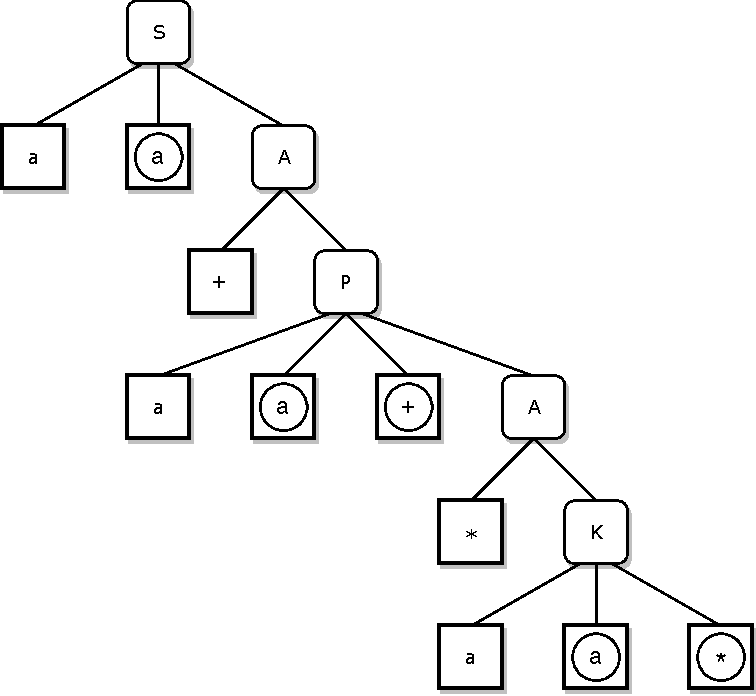
\includegraphics[width=0.8\linewidth]{img/PrekladovaGramatika}
		\caption{Ukázka překladové gramatiky}
		\label{fig:translateGrammar}
	\end{figure}
	\begin{figure}				
		\centering
		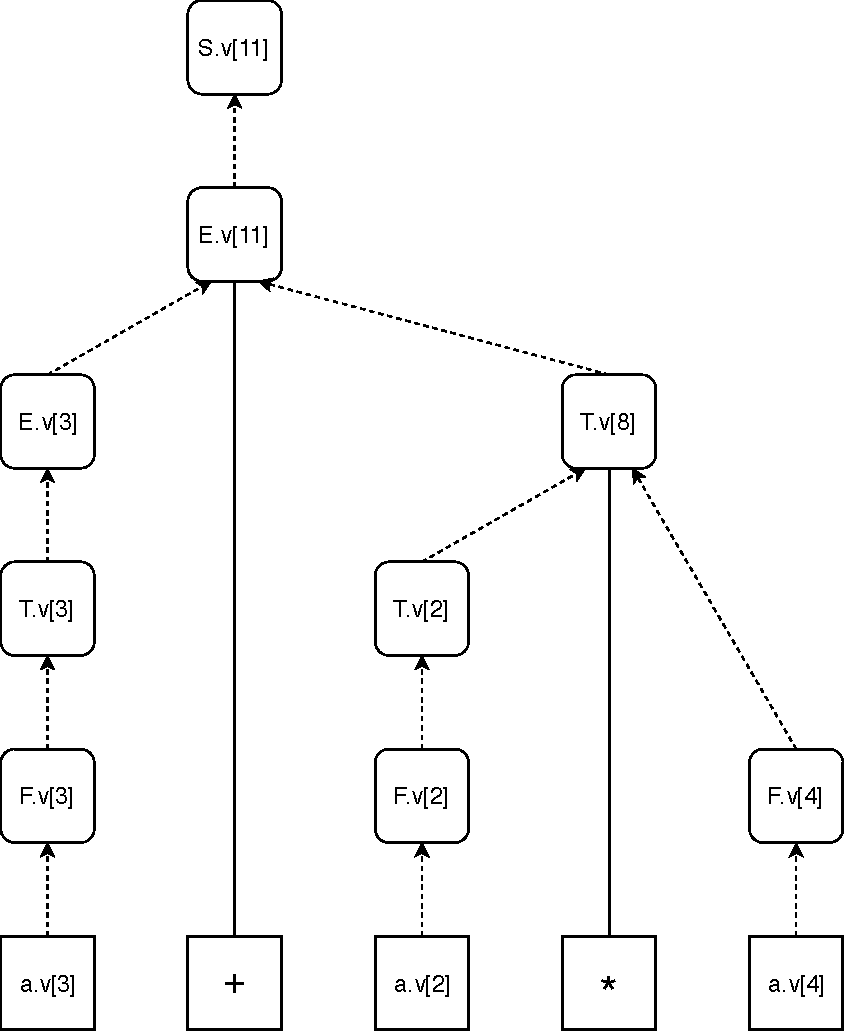
\includegraphics[width=0.8\linewidth]{img/AttributedArithmetic}
		\caption{Vyhodnocení atributů u atributované gramatiky}
		\label{fig:attributedGrammar}
	\end{figure}

	\begin{figure}				
		\centering
		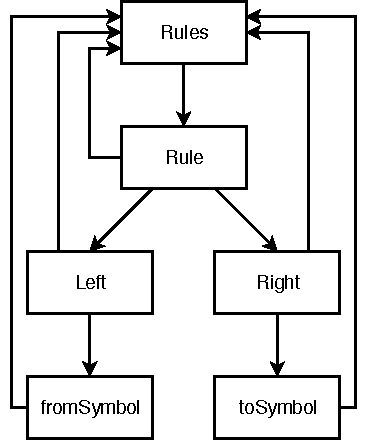
\includegraphics[width=0.4\linewidth]{img/RuleComputing}
		\caption{Výpočet vlastností pro třídu \Code{Rule}}
		\label{fig:ruleComputing}
	\end{figure}

	\begin{figure}				
		\centering
		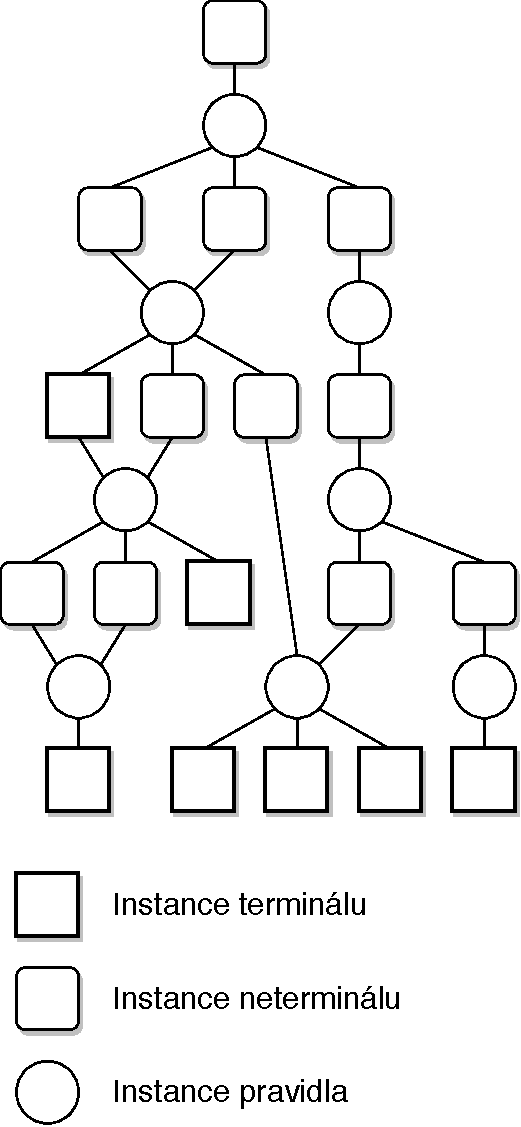
\includegraphics[width=0.6\linewidth]{img/Type0parsing}
		\caption{Reprezentace syntaktického stromu pro neomezené gramatiky}
		\label{fig:type0Parsing}
	\end{figure}

	\begin{figure}				
		\centering
		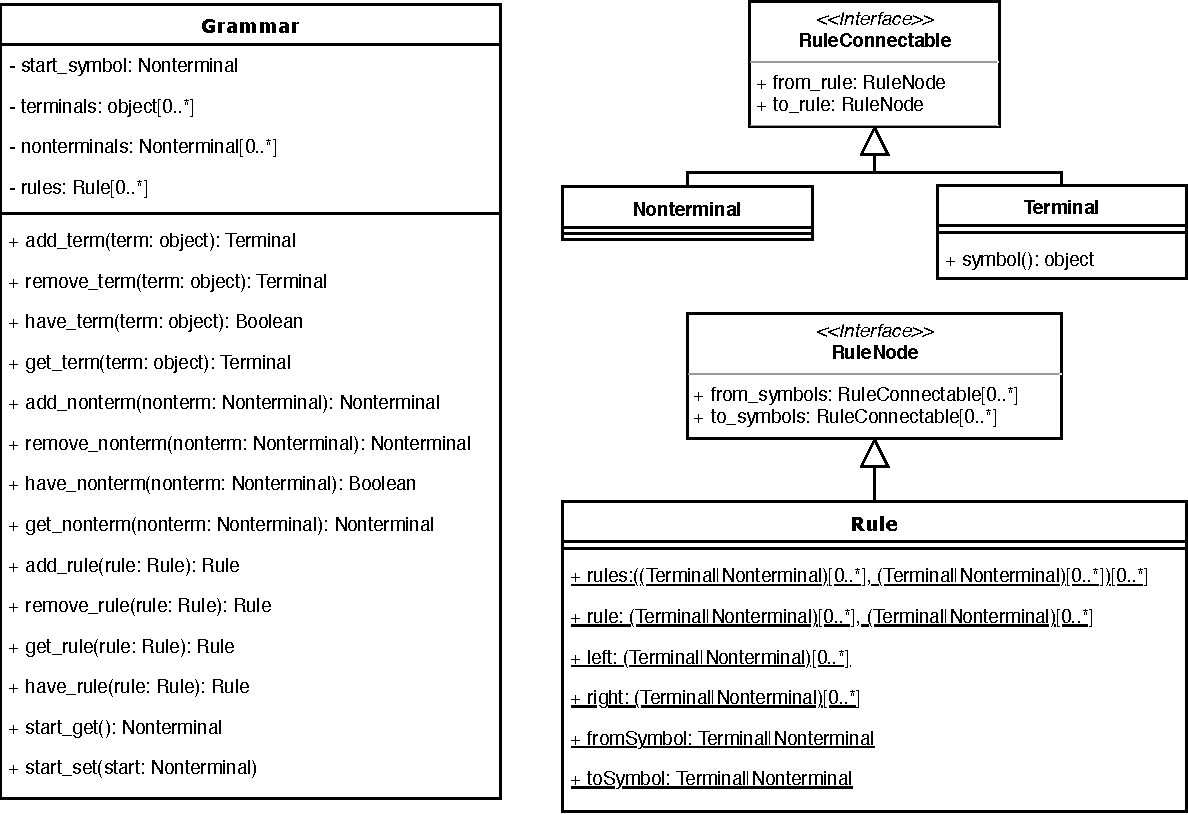
\includegraphics[width=0.9\linewidth]{img/WholeGrammpy}
		\caption{Kompletní návrh reprezentující gramatiku}
		\label{fig:grammpyWhole}
	\end{figure}

	\begin{figure}				
		\centering
		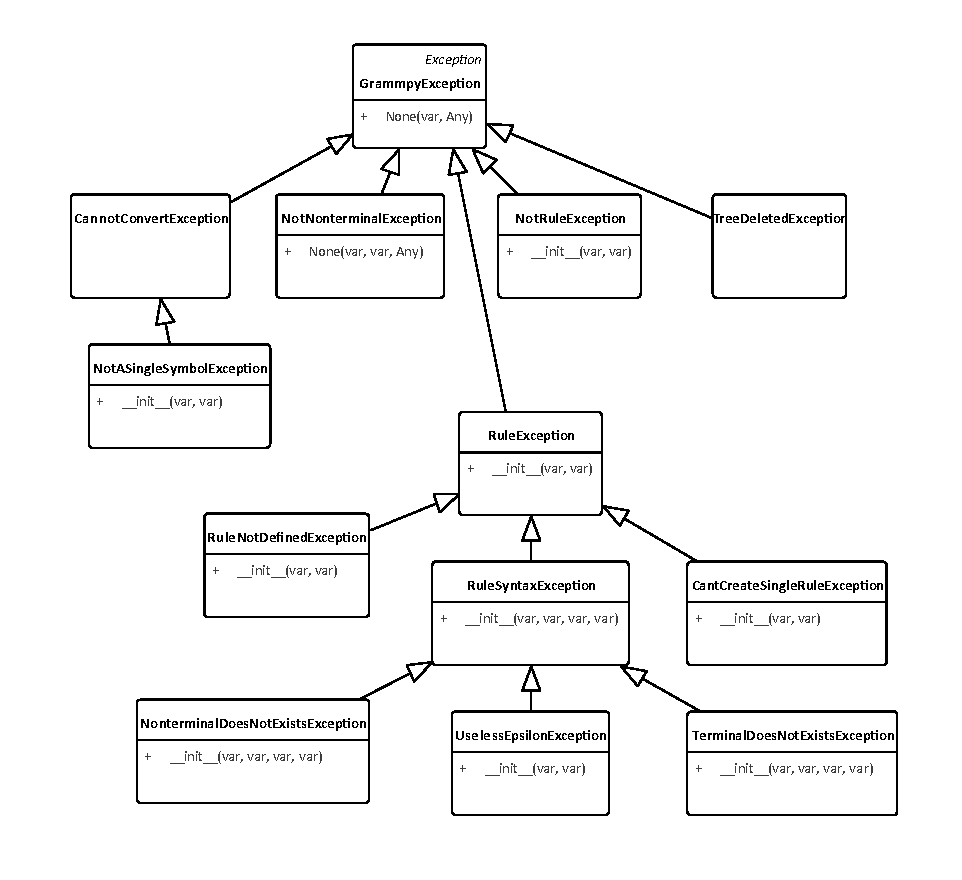
\includegraphics[width=0.8\linewidth]{img/grammpyExceptions}
		\caption{Hiearchie vyjímek v~modulu grammpy}
		\label{fig:grammpyExceptions}
	\end{figure}

	\begin{figure}				
		\centering
		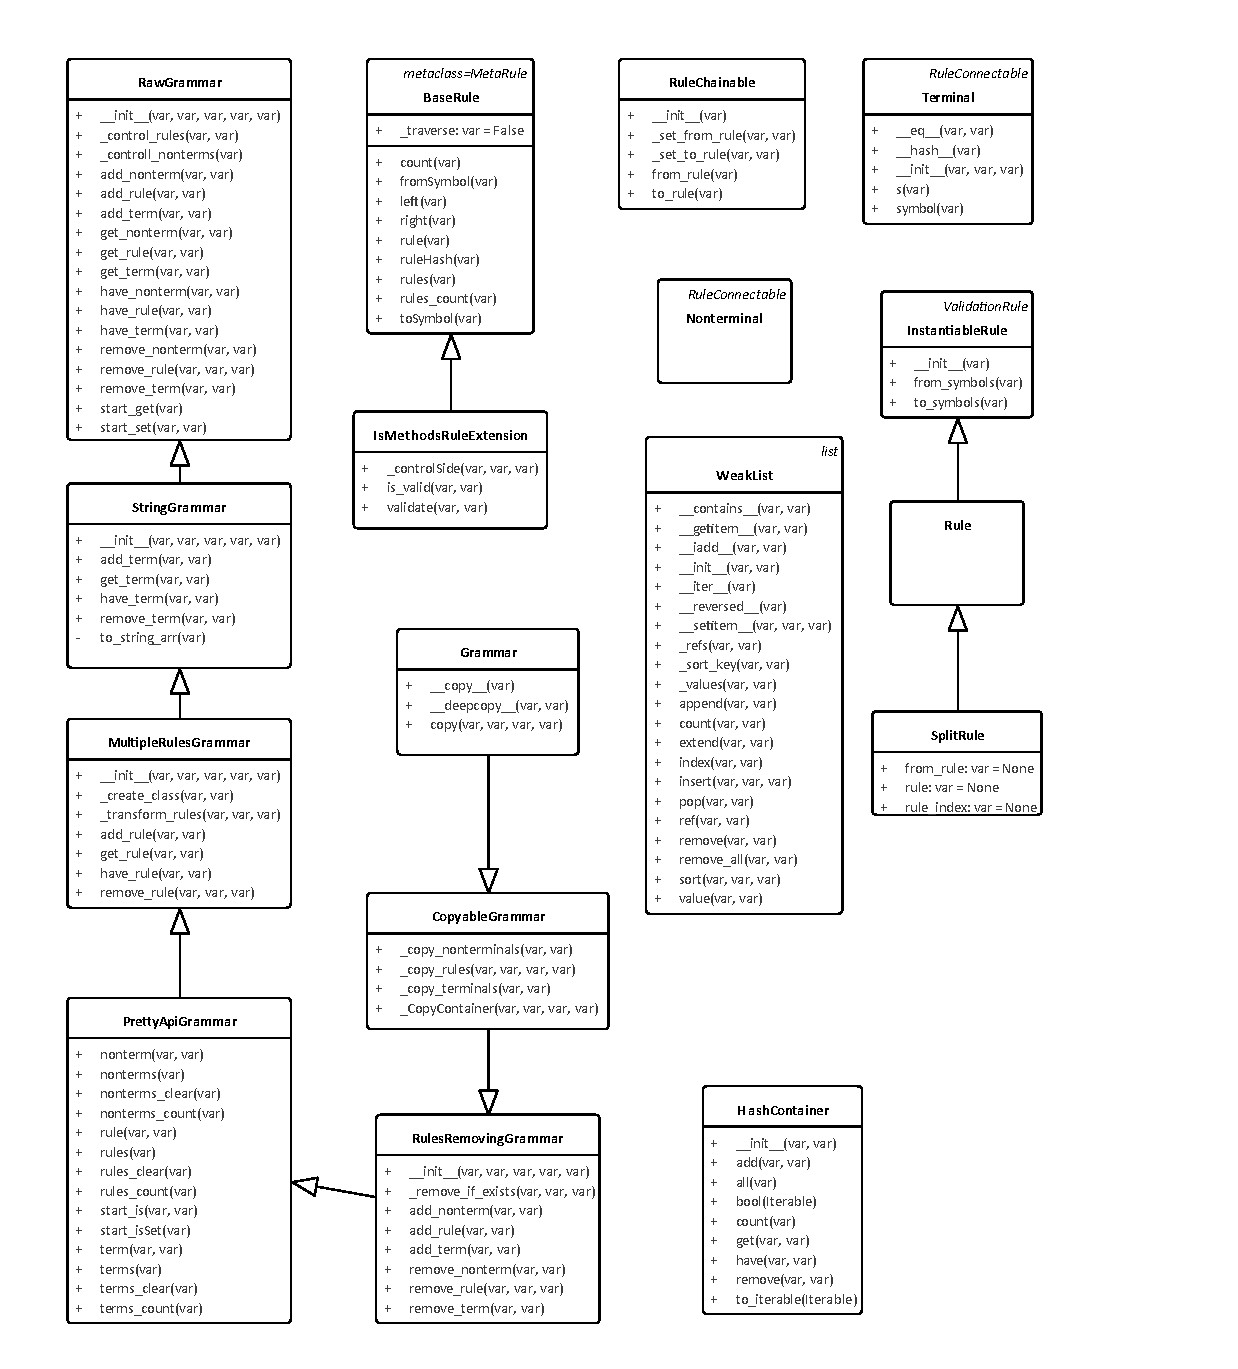
\includegraphics[width=\linewidth]{img/grammpyAPI}
		\caption{Class diagram implementace modulu grammpy}
		\label{fig:grammpyClasses}
	\end{figure}

	\begin{figure}				
		\centering
		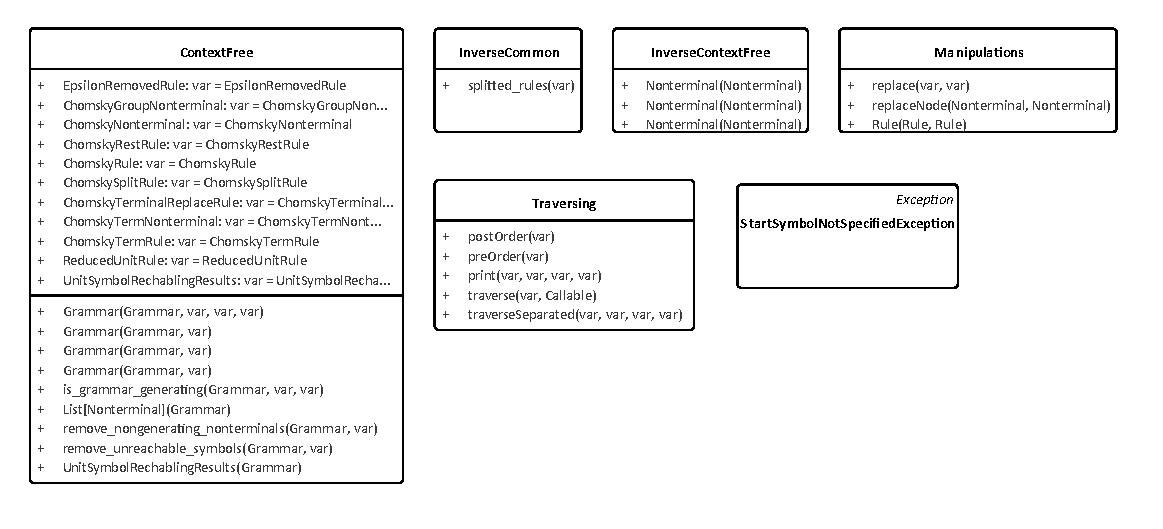
\includegraphics[width=\linewidth]{img/grammpy-transformsAPI}
		\caption{Class diagram implementace modulu grammpy-transforms}
		\label{fig:grammpyTransformsClasses}
	\end{figure}

	\begin{figure}				
		\centering
		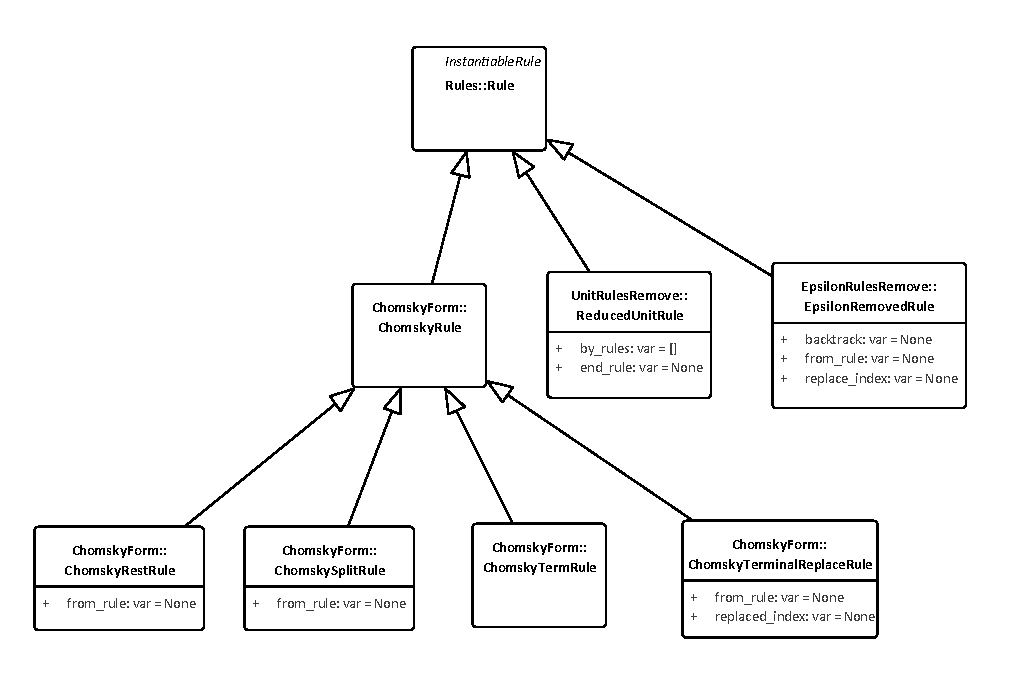
\includegraphics[width=0.8\linewidth]{img/grammpy-transformsRules}
		\caption{Class diagram pravidel v modulu grammpy-transforms}
		\label{fig:grammpyTransformsRules}
	\end{figure}

	\begin{figure}				
		\centering
		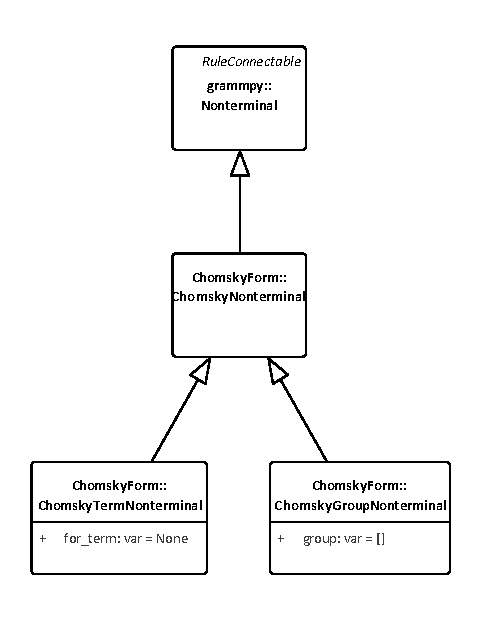
\includegraphics[width=0.4\linewidth]{img/grammpy-transformsNonterminals}
		\caption{Class diagram neterminálů v modulu grammpy-transforms}
		\label{fig:grammpyTransformsNonterminals}
	\end{figure}


\cleardoublepage
\printglossary[title=Seznam použitých zkratek]

\cleardoublepage
\chapter{Obsah přiloženého CD}
	\begin{figure}
		\dirtree{%
			.1 readme.txt\DTcomment{stručný popis obsahu CD}.
			.1 src.
				.2 grammpy\DTcomment{zdrojové kódy modulu grammpy}.
				.2 grammpy-transforms\DTcomment{zdrojové kódy modulu grammp-transforms}.
				.2 pyparsers\DTcomment{zdrojové kódy modulu pyparsers}.
			.1 examples\DTcomment{zdrojové kódy ukázek}.
				.2  lambda--cli\DTcomment{lambda kalkulus interpret}.
				.2  regex\_inverse\DTcomment{parser regulárních výrazů}.
				.2  calc\DTcomment{parser matematických výrazů}.
			.1 BP\_Valkovic\_Patrik\_2018.pdf\DTcomment{text práce ve formátu PDF}.
			.1 thesis\DTcomment{zdrojové soubory práce ve formátu \LaTeX}.
		}
	\end{figure}

\end{document}
